\documentclass[]{article}
\usepackage{lmodern}
\usepackage{amssymb,amsmath}
\usepackage{ifxetex,ifluatex}
\usepackage{fixltx2e} % provides \textsubscript
\ifnum 0\ifxetex 1\fi\ifluatex 1\fi=0 % if pdftex
  \usepackage[T1]{fontenc}
  \usepackage[utf8]{inputenc}
\else % if luatex or xelatex
  \ifxetex
    \usepackage{xltxtra,xunicode}
  \else
    \usepackage{fontspec}
  \fi
  \defaultfontfeatures{Ligatures=TeX,Scale=MatchLowercase}
\fi
% use upquote if available, for straight quotes in verbatim environments
\IfFileExists{upquote.sty}{\usepackage{upquote}}{}
% use microtype if available
\IfFileExists{microtype.sty}{%
\usepackage{microtype}
\UseMicrotypeSet[protrusion]{basicmath} % disable protrusion for tt fonts
}{}
\usepackage[a4paper]{geometry}
\usepackage[unicode=true]{hyperref}
\hypersetup{
            pdftitle={如何用 R Markdown 写学术文档?},
            pdfauthor={Shujia Wong},
            pdfborder={0 0 0},
            breaklinks=true}
\urlstyle{same}  % don't use monospace font for urls
\usepackage{natbib}
\bibliographystyle{apalike}
\usepackage{color}
\usepackage{fancyvrb}
\newcommand{\VerbBar}{|}
\newcommand{\VERB}{\Verb[commandchars=\\\{\}]}
\DefineVerbatimEnvironment{Highlighting}{Verbatim}{commandchars=\\\{\}}
% Add ',fontsize=\small' for more characters per line
\usepackage{framed}
\definecolor{shadecolor}{RGB}{248,248,248}
\newenvironment{Shaded}{\begin{snugshade}}{\end{snugshade}}
\newcommand{\AlertTok}[1]{\textcolor[rgb]{0.94,0.16,0.16}{#1}}
\newcommand{\AnnotationTok}[1]{\textcolor[rgb]{0.56,0.35,0.01}{\textbf{\textit{#1}}}}
\newcommand{\AttributeTok}[1]{\textcolor[rgb]{0.77,0.63,0.00}{#1}}
\newcommand{\BaseNTok}[1]{\textcolor[rgb]{0.00,0.00,0.81}{#1}}
\newcommand{\BuiltInTok}[1]{#1}
\newcommand{\CharTok}[1]{\textcolor[rgb]{0.31,0.60,0.02}{#1}}
\newcommand{\CommentTok}[1]{\textcolor[rgb]{0.56,0.35,0.01}{\textit{#1}}}
\newcommand{\CommentVarTok}[1]{\textcolor[rgb]{0.56,0.35,0.01}{\textbf{\textit{#1}}}}
\newcommand{\ConstantTok}[1]{\textcolor[rgb]{0.00,0.00,0.00}{#1}}
\newcommand{\ControlFlowTok}[1]{\textcolor[rgb]{0.13,0.29,0.53}{\textbf{#1}}}
\newcommand{\DataTypeTok}[1]{\textcolor[rgb]{0.13,0.29,0.53}{#1}}
\newcommand{\DecValTok}[1]{\textcolor[rgb]{0.00,0.00,0.81}{#1}}
\newcommand{\DocumentationTok}[1]{\textcolor[rgb]{0.56,0.35,0.01}{\textbf{\textit{#1}}}}
\newcommand{\ErrorTok}[1]{\textcolor[rgb]{0.64,0.00,0.00}{\textbf{#1}}}
\newcommand{\ExtensionTok}[1]{#1}
\newcommand{\FloatTok}[1]{\textcolor[rgb]{0.00,0.00,0.81}{#1}}
\newcommand{\FunctionTok}[1]{\textcolor[rgb]{0.00,0.00,0.00}{#1}}
\newcommand{\ImportTok}[1]{#1}
\newcommand{\InformationTok}[1]{\textcolor[rgb]{0.56,0.35,0.01}{\textbf{\textit{#1}}}}
\newcommand{\KeywordTok}[1]{\textcolor[rgb]{0.13,0.29,0.53}{\textbf{#1}}}
\newcommand{\NormalTok}[1]{#1}
\newcommand{\OperatorTok}[1]{\textcolor[rgb]{0.81,0.36,0.00}{\textbf{#1}}}
\newcommand{\OtherTok}[1]{\textcolor[rgb]{0.56,0.35,0.01}{#1}}
\newcommand{\PreprocessorTok}[1]{\textcolor[rgb]{0.56,0.35,0.01}{\textit{#1}}}
\newcommand{\RegionMarkerTok}[1]{#1}
\newcommand{\SpecialCharTok}[1]{\textcolor[rgb]{0.00,0.00,0.00}{#1}}
\newcommand{\SpecialStringTok}[1]{\textcolor[rgb]{0.31,0.60,0.02}{#1}}
\newcommand{\StringTok}[1]{\textcolor[rgb]{0.31,0.60,0.02}{#1}}
\newcommand{\VariableTok}[1]{\textcolor[rgb]{0.00,0.00,0.00}{#1}}
\newcommand{\VerbatimStringTok}[1]{\textcolor[rgb]{0.31,0.60,0.02}{#1}}
\newcommand{\WarningTok}[1]{\textcolor[rgb]{0.56,0.35,0.01}{\textbf{\textit{#1}}}}
\usepackage{longtable,booktabs}
% Fix footnotes in tables (requires footnote package)
\IfFileExists{footnote.sty}{\usepackage{footnote}\makesavenoteenv{long table}}{}
\IfFileExists{parskip.sty}{%
\usepackage{parskip}
}{% else
\setlength{\parindent}{0pt}
\setlength{\parskip}{6pt plus 2pt minus 1pt}
}
\setlength{\emergencystretch}{3em}  % prevent overfull lines
\providecommand{\tightlist}{%
  \setlength{\itemsep}{0pt}\setlength{\parskip}{0pt}}
\setcounter{secnumdepth}{5}
% Redefines (sub)paragraphs to behave more like sections
\ifx\paragraph\undefined\else
\let\oldparagraph\paragraph
\renewcommand{\paragraph}[1]{\oldparagraph{#1}\mbox{}}
\fi
\ifx\subparagraph\undefined\else
\let\oldsubparagraph\subparagraph
\renewcommand{\subparagraph}[1]{\oldsubparagraph{#1}\mbox{}}
\fi

% set default figure placement to htbp
\makeatletter
\def\fps@figure{htbp}
\makeatother

\usepackage[boldfont,slantfont]{xeCJK}
\usepackage{multicol}

\setmainfont{Times New Roman}
\setCJKmainfont[BoldFont={SimHei},ItalicFont={KaiTi}]{SimSun}
\setsansfont{SimHei}

\setCJKfamilyfont{song}{SimSun}
\setCJKfamilyfont{kai}{KaiTi}
\setCJKfamilyfont{hei}{SimHei}
\setCJKfamilyfont{yao}{FZYaoTi}

\newcommand\song{\CJKfamily{song}}
\newcommand\kai{\CJKfamily{kai}}
\newcommand\hei{\CJKfamily{hei}}
\newcommand\yao{\CJKfamily{yao}}

\newcommand{\erhao}{\fontsize{22pt}{\baselineskip}\selectfont}
\newcommand{\xiaoerhao}{\fontsize{18pt}{\baselineskip}\selectfont}
\newcommand{\sanhao}{\fontsize{16pt}{\baselineskip}\selectfont}
\newcommand{\xiaosanhao}{\fontsize{15pt}{\baselineskip}\selectfont}
\newcommand{\sihao}{\fontsize{14pt}{\baselineskip}\selectfont}
\newcommand{\xiaosihao}{\fontsize{12pt}{\baselineskip}\selectfont}
\newcommand{\wuhao}{\fontsize{10.5pt}{\baselineskip}\selectfont}
\newcommand{\xiaowuhao}{\fontsize{9pt}{\baselineskip}\selectfont}
\newcommand{\liuhao}{\fontsize{7.5pt}{\baselineskip}\selectfont}

%%%段落首行缩进两个字
\makeatletter
\let\@afterindentfalse\@afterindenttrue
\@afterindenttrue
\makeatother
\setlength{\parindent}{2em}%中文缩进两个汉字位

%%%%%%%%%% 定理类环境的定义 %%%%%%%%%%
%% 必须在导入中文环境之后
\newtheorem{example}{例}             % 整体编号
\newtheorem{algorithm}{算法}
\newtheorem{theorem}{定理}[section]  % 按 section 编号
\newtheorem{definition}{定义}
\newtheorem{axiom}{公理}
\newtheorem{property}{性质}
\newtheorem{proposition}{命题}
\newtheorem{lemma}{引理}
\newtheorem{corollary}{推论}
\newtheorem{remark}{注解}
\newtheorem{condition}{条件}
\newtheorem{conclusion}{结论}
\newtheorem{assumption}{假设}

%%%%%%%%%% 一些重定义 %%%%%%%%%%
%% 必须在导入中文环境之后
\renewcommand{\contentsname}{目录}     % 将Contents改为目录
\renewcommand{\abstractname}{摘\ \ 要} % 将Abstract改为摘要
\renewcommand{\refname}{参考文献}      % 将References改为参考文献
\renewcommand{\indexname}{索引}
\renewcommand{\figurename}{图}
\renewcommand{\tablename}{表}
\renewcommand{\appendixname}{附录}
%\renewcommand{\proofname}{证明}
\renewcommand{\algorithm}{算法}

%%%%%%%%%%%%%%%%%%%%%%%%%%%%%%%%%%%%%%%%%%%%%%%%%%%%%%%%%%%%%%%%
%  packages
%    这部分声明需要用到的包
%%%%%%%%%%%%%%%%%%%%%%%%%%%%%%%%%%%%%%%%%%%%%%%%%%%%%%%%%%%%%%%%
\usepackage{graphicx}    % EPS 图片支持
\usepackage{indentfirst} % 中文段落首行缩进
\usepackage{bm}          % 公式中的粗体字符(用命令\boldsymbol)

%%%%%%%%%%%%%%%%%%%%%%%%%%%%%%%%%%%%%%%%%%%%%%%%%%%%%%%%%%%%%%%%
%  lengths
%    下面的命令重定义页面边距,使其符合中文刊物习惯。
%%%%%%%%%%%%%%%%%%%%%%%%%%%%%%%%%%%%%%%%%%%%%%%%%%%%%%%%%%%%%%%%
\addtolength{\topmargin}{-54pt}
\setlength{\oddsidemargin}{0.63cm}  % 3.17cm - 1 inch
\setlength{\evensidemargin}{\oddsidemargin}
\setlength{\textwidth}{14.66cm}
\setlength{\textheight}{24.00cm}    % 24.62


\title{{\hei{如何用 R Markdown 写学术文档?}}}
\author{Shujia Wong}
\date{}

\let\BeginKnitrBlock\begin \let\EndKnitrBlock\end
\begin{document}
\maketitle

\begin{center}
\parbox{\textwidth}{
%\rule{2em}{0pt}
\hei{摘要:}\song{
这算是用R Markdown学习R和写作的学习笔记吧。
主要包括:
1.用Rmarkdown写科研笔记或一般学术文档;
2.用bookdown写书或论文;
3.记录Rmarkdown的一些用法。
}\\[5pt]

\hei{关键词:}\song{
Rmarkdown;bookdown;bookdownplus
}
\\[5pt]
}
\end{center}

%%%%%%%%%%%%%%%%%%%%%%%%%%%%%%%%%%%%%%%%%%%%%%%%%%%%%%%%%%%%%%%%
%  英文摘要
%%%%%%%%%%%%%%%%%%%%%%%%%%%%%%%%%%%%%%%%%%%%%%%%%%%%%%%%%%%%%%%%

%%{
%\setcounter{tocdepth}{2}
%\tableofcontents
%}
%
\section{介绍}

\hypertarget{r-markdown}{%
\subsection{什么是R Markdown?}\label{r-markdown}}

R Markdown \citep{R-rmarkdown}
是结合Markdown和R\citep{R-base}语言的写作软件。

Markdown是轻量级、纯文本、超简单的书写格式。

R Markdown可以做什么?

\begin{itemize}
\tightlist
\item
  语法简单。作者基本上无需关心排版问题,只要专心写作就可以了。
\item
  计算结果动态生成。作者不必手动拷贝粘贴代码结果或者生成的表格、图片等。
\item
  易于修改。写作过程中如需修改某处,全文相应变动会自动生成,包括软件运行的结果(图形等)。
\item
  比Word更美观,比LaTeX更易用。
\item
  方便地插入目录、图表、脚注等。Bookdown扩展功能可以交叉引用、索引。
\item
  方便地插入数学公式、参考文献、R代码。
\item
  可以生成漂亮的pdf、word、epub、网页和幻灯片等多种文件格式。
\item
  写作及结果具有可重复性。
\item
  支持多语言,包括 R, C/C++, Python, Fortran, Julia, Shell scripts和
  SQL等。
\item
  R 和 Markdown 都是开源免费的。
\end{itemize}

Rmarkdown 使得数据分析代码可以与文档混编,具体语法请参看《R
Markdown语法简介》。

下面是回归模型的简单例子。在R中,回归模型可以用非常简单的一行代码搞定:\texttt{lm(y\textasciitilde{}x,\ data)},

\begin{Shaded}
\begin{Highlighting}[]
\KeywordTok{options}\NormalTok{(}\DataTypeTok{digits =} \DecValTok{4}\NormalTok{)}
\NormalTok{fit =}\StringTok{ }\KeywordTok{lm}\NormalTok{(dist }\OperatorTok{~}\StringTok{ }\NormalTok{speed, }\DataTypeTok{data =}\NormalTok{ cars)}
\KeywordTok{coef}\NormalTok{(}\KeywordTok{summary}\NormalTok{(fit))}
\end{Highlighting}
\end{Shaded}

\begin{verbatim}
            Estimate Std. Error t value  Pr(>|t|)
(Intercept)  -17.579     6.7584  -2.601 1.232e-02
speed          3.932     0.4155   9.464 1.490e-12
\end{verbatim}

\begin{Shaded}
\begin{Highlighting}[]
\NormalTok{b =}\StringTok{ }\KeywordTok{coef}\NormalTok{(fit)}
\end{Highlighting}
\end{Shaded}

上面回归方程中的斜率是3.9324,完整的回归方程为:\[ Y = -17.5791 + 3.9324x\]

散点图和回归直线(见图\ref{fig:scatter}):

\begin{Shaded}
\begin{Highlighting}[]
\KeywordTok{par}\NormalTok{(}\DataTypeTok{mar =} \KeywordTok{c}\NormalTok{(}\DecValTok{4}\NormalTok{, }\DecValTok{4}\NormalTok{, }\FloatTok{.1}\NormalTok{, }\FloatTok{.1}\NormalTok{), }\DataTypeTok{las =} \DecValTok{1}\NormalTok{)}
\KeywordTok{plot}\NormalTok{(cars, }\DataTypeTok{pch =} \DecValTok{19}\NormalTok{)}
\KeywordTok{abline}\NormalTok{(fit, }\DataTypeTok{col =} \StringTok{'red'}\NormalTok{)}
\end{Highlighting}
\end{Shaded}

\begin{figure}

{\centering 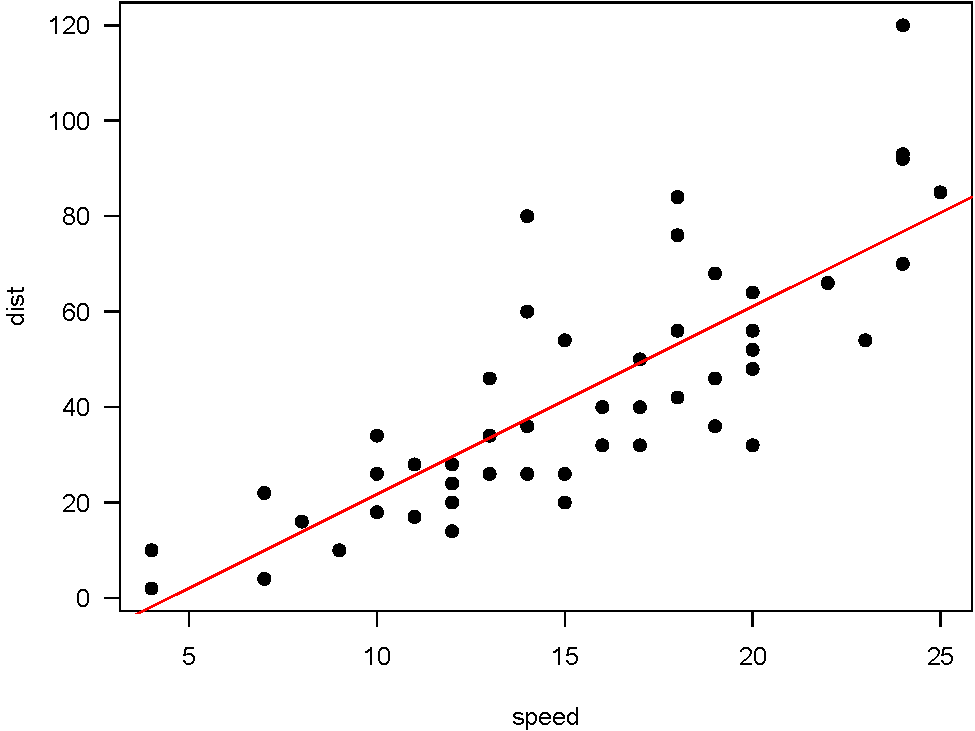
\includegraphics[width=0.75\linewidth]{article_zh_files/figure-latex/scatter-1} 

}

\caption{cars数据散点图以及回归直线。}\label{fig:scatter}
\end{figure}

\subsection{系统环境}

需要安装的软件:

\begin{itemize}
\item
  R:\url{https://www.r-project.org/}
\item
  RStudio:\url{https://www.rstudio.com/}
\item
  Bookdown:\url{https://bookdown.org/}
\end{itemize}

安装Bookdown
\citep{R-bookdown}及其相依软件包基本上就OK了,包括了rmarkdown
\citep{R-rmarkdown}、knitr \citep{R-knitr}、
rticles等,如果有缺失的,运行时会提示安装。

可以安装稳定版: \texttt{install.packages(’bookdown’)}

或开发版:
\texttt{devtools::install\_github(\textquotesingle{}rstudio/bookdown\textquotesingle{})}

\hypertarget{rstudio}{%
\subsection{RStudio基本设置}\label{rstudio}}

打开 Tools→global options,然后

\begin{itemize}
\item
  点击\texttt{sweave},在\texttt{weave\ rnw\ files\ using}选择
  \textbf{knitr}
\item
  在\texttt{Typeset\ LaTex\ into\ PDF\ using} 选择\textbf{XeLaTex}
\item
  在\texttt{Code\ -\textgreater{}\ Saving\ -\textgreater{}\ Default\ text\ Encoding}
  选择 \texttt{UTF-8}
\end{itemize}

\hypertarget{-r-markdown-}{%
\section{用 R Markdown 写简单学术文档}\label{-r-markdown-}}

所谓``简单''学术文档,是指满足了学术文档的基本要求,包括标题、公式、图表、参考文献以及自动编号等,但是不能交互引用。这种情况下
RMarkdown 具有独特优势,可以直接上手,输出结果丰富。

\begin{enumerate}
\def\labelenumi{\arabic{enumi}.}
\item
  新建一个R Markdown
  文档。在打开界面可输入题目和作者姓名,输出格式可选择\texttt{html},\texttt{pdf}
  或 \texttt{word}。
\item
  简单设置。点击\texttt{Knit}旁边的齿轮按钮,在\texttt{Output\ Options}可做更多选择,比如可勾选\texttt{Include\ table\ of\ contents},表示建立目录。勾选\texttt{Number\ section\ headings}表示章节题目包含顺序数字。在\texttt{Figures}勾选\texttt{Render\ figure\ captions}表示图形会显示标题并自动排序。
\item
  结果输出。
\end{enumerate}

\begin{itemize}
\tightlist
\item
  如果文档是\textbf{纯英文}的,可以通过 \texttt{knit} 转为
  \texttt{html},\texttt{pdf} 或 \texttt{word}
  任何格式都没问题。不过,如果你用中文Windows,则日期最好用
  \texttt{"\textasciigrave{}\ r\ Sys.Date()\ \textasciigrave{}"}
  代替或直接输入英文日期,否则可能会乱码。
\item
  如果文档是\textbf{中文}的,则

  \begin{itemize}
  \tightlist
  \item
    转 \texttt{html} 没有任何问题。
  \item
    转\texttt{word},一定要在开始时指定,或在文档的\texttt{output:}下面指明\texttt{word\_document:},否则标题和日期会是乱码。
  \item
    中文文档不能直接转\texttt{pdf}。
  \end{itemize}
\end{itemize}

\textbf{中文文档如何转\texttt{pdf}?}

要转为 pdf文档,必须安装软件包\texttt{rticles}。用法很简单:打开
Rmarkdown时,选择 \texttt{From\ Template},从模版中选择
\texttt{CTex\ Documents}即可。

一般文档开头(称为\texttt{yaml})是这样的:

\begin{Shaded}
\begin{Highlighting}[]
\NormalTok{---}
\NormalTok{title: "你的论文题目"}
\NormalTok{author: "你的姓名"}
\NormalTok{date:  "2018-09-17"}
\NormalTok{output: }
\NormalTok{  html_document:                           #文档格式为html}
\BaseNTok{    fig_caption: yes                       #包括图形标题}
\BaseNTok{    number_sections: yes                   #章节数字顺序}
\BaseNTok{    toc: yes                               #显示目录}
\BaseNTok{    toc_depth: 3                           #三级目录}
\BaseNTok{    toc_float: True                        #目录作为侧边栏}
\NormalTok{bibliography: reference.bib                #参考文献文件名}
\NormalTok{bibli0-style: apalike                      #参考文献格式}
\NormalTok{link-citations: yes                        #参考文献链接}
\NormalTok{colorlinks: yes                            #链接颜色}
\NormalTok{#lot: yes                                  #表格列表}
\NormalTok{#lof: yes                                  #图形列表}
\NormalTok{---}
\end{Highlighting}
\end{Shaded}

\hypertarget{-r-markdown-}{%
\section{用 R Markdown 写学术文档}\label{-r-markdown-}}

前面介绍的R
Markdown文档是没有\textbf{交叉引用}功能的,即公式、图形、表格或章节之间在正文的引用不能自动编号。

为了实现交叉引用功能,可以扩展到\texttt{bookdown}。

\textbf{撰写可以交叉引用的网页文档}:

把\texttt{html\_document:}换成\texttt{bookdown::html\_document2:}即可,其它不变。

\textbf{撰写可以交叉引用的pdf文档}:

如果文档是\textbf{纯英文}的,把\texttt{html\_document:}换成\texttt{bookdown::pdf\_document2:}即可,其它不变。
如果文档含有中文字符,还是老老实实用软件包bookdown或bookdownplus吧。

\textbf{撰写可以交叉引用的docx文档}:

一样把\texttt{word\_document:}换成\texttt{bookdown::word\_document2:}。但是直接产生的word文档格式不一定满足要求,如标题是蓝色的等等。

可以制作一个\textbf{参考文档}:由R Markdown产生一个
word文档,然后对该文档的\textbf{样式}进行编辑(编辑其它功能无效)。

我已经编辑了一个参考文档:word\_style.docx,你可以结合需要自行再通过\emph{样式}修改。

我的 \texttt{yaml}是这样的:

\begin{Shaded}
\begin{Highlighting}[]
\NormalTok{---}
\NormalTok{title: "Word 参考文档"}
\NormalTok{author:}
\NormalTok{  - WSJ}
\NormalTok{  - College of Economics,Shenzhen University}
\NormalTok{date:  "2018-09-17"}
\NormalTok{output:}
\NormalTok{  bookdown::word_document2: }
\BaseNTok{    reference_docx: template/word_style.docx}
\BaseNTok{    fig_caption: yes}
\NormalTok{bibliography: [bib/packages.bib,bib/book.bib]}
\NormalTok{csl: csl/chinese-gb7714-1987-numeric.csl}
\NormalTok{#bibli0-style: apalike}
\NormalTok{link-citations: yes}
\NormalTok{colorlinks: yes}
\NormalTok{#lot: yes}
\NormalTok{#lof: yes}
\NormalTok{---}
\end{Highlighting}
\end{Shaded}

\textbf{如何修改参考文献格式?}

注释掉 \texttt{\#bibli0-style:\ apalike}, 然后增加一行:

csl: csl/chinese-gb7714-1987-numeric.csl

\hypertarget{bookdown}{%
\section{用Bookdown写书或长文}\label{bookdown}}

长篇论文(书籍、毕业论文)需要分章节以及交叉引用,结构复杂,简单的一个Rmarkdown文档可能不能胜任。

一本 \textbf{bookdown} 书含有多个章节,每个章节写在单独的\texttt{.Rmd}
文件,起始部分为该章节标题 \texttt{\#\ Chapter\ Title}。

如果含有中文,所有 R Markdown 文档都必须用 UTF-8编码保存。

以下是一本书的典型例子:

\begin{itemize}
\item
  index.Rmd

\begin{Shaded}
\begin{Highlighting}[]
\FunctionTok{# Preface \{-\}}

\NormalTok{In this book, we will introduce an interesting}
\NormalTok{method.}
\end{Highlighting}
\end{Shaded}
\item
  01-intro.Rmd

\begin{Shaded}
\begin{Highlighting}[]
\FunctionTok{# Introduction}

\NormalTok{This chapter is an overview of the methods that}
\NormalTok{we propose to solve an **important problem**.}
\end{Highlighting}
\end{Shaded}
\item
  02-literature.Rmd

\begin{Shaded}
\begin{Highlighting}[]
\FunctionTok{# Literature}

\NormalTok{Here is a review of existing methods.}
\end{Highlighting}
\end{Shaded}
\item
  03-method.Rmd

\begin{Shaded}
\begin{Highlighting}[]
\FunctionTok{# Methods}

\NormalTok{We describe our methods in this chapter.}
\end{Highlighting}
\end{Shaded}
\item
  04-application.Rmd

\begin{Shaded}
\begin{Highlighting}[]
\FunctionTok{# Applications}

\NormalTok{Some _significant_ applications are demonstrated}
\NormalTok{in this chapter.}

\FunctionTok{## Example one}

\FunctionTok{## Example two}
\end{Highlighting}
\end{Shaded}
\item
  05-summary.Rmd

\begin{Shaded}
\begin{Highlighting}[]
\FunctionTok{# Final Words}

\NormalTok{We have finished a nice book.}
\end{Highlighting}
\end{Shaded}
\end{itemize}

\textbf{具体用法}:

\begin{itemize}
\tightlist
\item
  下载模板:在模板下载网页(github)的右上角,点击\texttt{Clone\ or\ download}
  下载压缩文件,解压到工作目录。

  \begin{itemize}
  \tightlist
  \item
    英文模版 \url{https://github.com/rstudio/bookdown-demo}。
  \item
    中文模版https://github.com/yihui/bookdown-chinese
  \end{itemize}
\item
  用RStudio打开文件\texttt{bookdown-demo.Rproj}或\texttt{bookdown-chinese.Rproj},然后在右上角点击\texttt{Build},下一行\texttt{Build\ Book},然后选择相应格式
  (pdf,epub,word,gitbook) 即可得到模板文件。
\item
  根据自己需要修改相关文件,保存。运行\texttt{Build\ Book}即可得到你自己的书籍。
\end{itemize}

其中中文书可输出格式 \texttt{gitbook}网页、\texttt{pdf}, \texttt{word}
和 \texttt{epub}。

英文的demo里默认没有
\texttt{word}格式的输出,要自行在\texttt{\_output.yml}里添加一行:

\texttt{bookdown::word\_document2:\ default}

更多说明请参看 Xie Yihui(2018):\emph{bookdown: Authoring Books and
Technical Documents with R Markdown}
(\url{https://bookdown.org/yihui/bookdown/})

\hypertarget{-bookdownplus-}{%
\section{用 Bookdownplus 模版快速上手}\label{-bookdownplus-}}

Bookdownplus\citep{R-bookdownplus}
对Bookdown进行了重新配置,制作了多种文本的模版,包括中、英文论文,北大、浙大等高校毕业论文等,大大方便了各种类型的写作应用。

\subsection{安装调用}

软件包bookdownplus 可参看 \texttt{CRAN}
\url{https://cran.r-project.org/web/packages/bookdownplus/index.html}。
也可以到\texttt{Github} \url{https://github.com/pzhaonet/bookdownplus}
去下载相关文件。

安装稳定版:\texttt{install.packages(’bookdownplus’)}

或开发版:\texttt{devtools::install\_github(\textquotesingle{}pzhaonet/bookdownplus\textquotesingle{})}

调用软件包:

\begin{Shaded}
\begin{Highlighting}[]
\KeywordTok{require}\NormalTok{(bookdownplus)}
\end{Highlighting}
\end{Shaded}

查看所有可用模版:

\begin{Shaded}
\begin{Highlighting}[]
\KeywordTok{template}\NormalTok{()}
\NormalTok{ [}\DecValTok{1}\NormalTok{] }\StringTok{"article"}         \StringTok{"article_mdpi"}    \StringTok{"article_zh"}     
\NormalTok{ [}\DecValTok{4}\NormalTok{] }\StringTok{"calendar"}        \StringTok{"cchess"}          \StringTok{"chemistry"}      
\NormalTok{ [}\DecValTok{7}\NormalTok{] }\StringTok{"chemistry_zh"}    \StringTok{"discussion"}      \StringTok{"dnd_dev"}        
\NormalTok{[}\DecValTok{10}\NormalTok{] }\StringTok{"docsens"}         \StringTok{"guitar"}          \StringTok{"igo"}            
\NormalTok{[}\DecValTok{13}\NormalTok{] }\StringTok{"journal"}         \StringTok{"mail"}            \StringTok{"musix"}          
\NormalTok{[}\DecValTok{16}\NormalTok{] }\StringTok{"nonpar"}          \StringTok{"nte_zh"}          \StringTok{"poem"}           
\NormalTok{[}\DecValTok{19}\NormalTok{] }\StringTok{"poster"}          \StringTok{"rbasics"}         \StringTok{"skak"}           
\NormalTok{[}\DecValTok{22}\NormalTok{] }\StringTok{"thesis_classic"}  \StringTok{"thesis_mypku_zh"} \StringTok{"thesis_pku_zh"}  
\NormalTok{[}\DecValTok{25}\NormalTok{] }\StringTok{"thesis_ubt"}      \StringTok{"thesis_zju_zh"}   \StringTok{"yihui_crc"}      
\NormalTok{[}\DecValTok{28}\NormalTok{] }\StringTok{"yihui_demo"}      \StringTok{"yihui_mini"}      \StringTok{"yihui_zh"}       
\end{Highlighting}
\end{Shaded}

其中 \texttt{article} 是英文版学术论文模版,\texttt{article\_zh}
是中文学术论文模版,\texttt{thesis\_pku\_zh}
是北京大学毕业论文模版,\texttt{thesis\_zju\_zh} 是浙江大学的。

\hypertarget{R-mark}{%
\section{R Markdown简介}\label{R-mark}}

\subsection{基本语法}

\subsubsection{行内语法}

\begin{itemize}
\tightlist
\item
  斜体: \emph{text},\texttt{\_text\_} or \texttt{*text*}
\item
  黑体:\textbf{text},\texttt{\_\_text\_\_} or \texttt{**text**}
\item
  下标:两个\texttt{\textasciitilde{}}包夹,\texttt{H\textasciitilde{}2\textasciitilde{}SO\textasciitilde{}4\textasciitilde{}}
  renders H\textsubscript{2}SO\textsubscript{4}
\item
  上标:两个\texttt{\^{}}包夹, \texttt{R\^{}2\^{}} renders
  R\textsuperscript{2}
\item
  显示代码:\texttt{code}和\texttt{code}显示代码块
\item
  行内运行R代码:\texttt{10}, 100的开根号等于 10
\item
  链接网站:\texttt{{[}text{]}(link)},例如
  \href{https://www.rstudio.com}{RStudio}
\item
  插入图片:\texttt{!{[}image\ title{]}(path/to/image)}
\item
  脚注:\texttt{\^{}{[}{]}}, e.g., 这里是脚注\footnote{This is a
    footnote.}
\end{itemize}

\subsubsection{模块语法}

Section headers can be written after a number of pound signs, e.g.,

\begin{Shaded}
\begin{Highlighting}[]
\FunctionTok{# First-level header}
\FunctionTok{## Second-level header}
\FunctionTok{### Third-level header}
\end{Highlighting}
\end{Shaded}

If you do not want a certain heading to be numbered, you can add
\texttt{\{-\}} after the heading, e.g.,

\begin{Shaded}
\begin{Highlighting}[]
\FunctionTok{# Preface \{-\}}
\end{Highlighting}
\end{Shaded}

Unordered list items start with \texttt{*}, \texttt{-}, or \texttt{+},
and you can nest one list within another list by indenting the sub-list
by four spaces, e.g.,

\begin{Shaded}
\begin{Highlighting}[]
\NormalTok{- }\FloatTok{one item}
\FloatTok{- one item}
\FloatTok{- one item}
\FloatTok{    - one item}
\FloatTok{    - one item}
\end{Highlighting}
\end{Shaded}

The output is:

\begin{itemize}
\tightlist
\item
  one item
\item
  one item
\item
  one item

  \begin{itemize}
  \tightlist
  \item
    one item
  \item
    one item
  \end{itemize}
\end{itemize}

Ordered list items start with numbers (the rule for nested lists is the
same as above), e.g.,

\begin{Shaded}
\begin{Highlighting}[]
\NormalTok{1. }\FloatTok{the first item}
\FloatTok{2. the second item}
\FloatTok{3. the third item}
\end{Highlighting}
\end{Shaded}

The output does not look too much different with the Markdown source:

\begin{enumerate}
\def\labelenumi{\arabic{enumi}.}
\tightlist
\item
  the first item
\item
  the second item
\item
  the third item
\end{enumerate}

Blockquotes are written after \texttt{\textgreater{}}, e.g.,

\begin{quote}
``I thoroughly disapprove of duels. If a man should challenge me, I
would take him kindly and forgivingly by the hand and lead him to a
quiet place and kill him.''

\begin{flushright}--- Mark Twain\end{flushright}
\end{quote}

Plain code blocks can be written after three or more backticks, and you
can also indent the blocks by four spaces, e.g.,

\begin{Shaded}
\begin{Highlighting}[]
\NormalTok{```}
\NormalTok{This text is displayed verbatim / preformatted}
\NormalTok{```}

\NormalTok{Or indent by four spaces:}

\BaseNTok{    This text is displayed verbatim / preformatted}
\end{Highlighting}
\end{Shaded}

\subsection{数学公式}

行内公式\texttt{\$y=x\^{}2\$}显示\(y=x^2\),整行公式(display
style)用两双美元符号之间表示,
\texttt{\$\$f(k)\ =\ \{n\ \textbackslash{}choose\ k\}\ p\^{}\{k\}\ (1-p)\^{}\{n-k\}\$\$},
结果:

\[f\left(k\right)=\binom{n}{k}p^k\left(1-p\right)^{n-k}\]

You can also use math environments inside \texttt{\$\ \$} or
\texttt{\$\$\ \$\$}, e.g.,

\begin{Shaded}
\begin{Highlighting}[]
\SpecialStringTok{$$}\SpecialCharTok{\textbackslash{}begin}\SpecialStringTok{\{array\}\{ccc\}}
\SpecialStringTok{x_\{11\} & x_\{12\} & x_\{13\}}\SpecialCharTok{\textbackslash{}\textbackslash{}}
\SpecialStringTok{x_\{21\} & x_\{22\} & x_\{23\}}
\SpecialCharTok{\textbackslash{}end}\SpecialStringTok{\{array\}$$}
\end{Highlighting}
\end{Shaded}

\[\begin{array}{ccc}
x_{11} & x_{12} & x_{13}\\
x_{21} & x_{22} & x_{23}
\end{array}\]

\begin{Shaded}
\begin{Highlighting}[]
\SpecialStringTok{$$X = }\SpecialCharTok{\textbackslash{}begin}\SpecialStringTok{\{bmatrix\}1 & x_\{1\}}\SpecialCharTok{\textbackslash{}\textbackslash{}}
\SpecialStringTok{1 & x_\{2\}}\SpecialCharTok{\textbackslash{}\textbackslash{}}
\SpecialStringTok{1 & x_\{3\}}
\SpecialCharTok{\textbackslash{}end}\SpecialStringTok{\{bmatrix\}$$}
\end{Highlighting}
\end{Shaded}

\[X = \begin{bmatrix}1 & x_{1}\\
1 & x_{2}\\
1 & x_{3}
\end{bmatrix}\]

\begin{Shaded}
\begin{Highlighting}[]
\SpecialStringTok{$$}\SpecialCharTok{\textbackslash{}Theta}\SpecialStringTok{ = }\SpecialCharTok{\textbackslash{}begin}\SpecialStringTok{\{pmatrix\}}\SpecialCharTok{\textbackslash{}alpha}\SpecialStringTok{ & }\SpecialCharTok{\textbackslash{}beta\textbackslash{}\textbackslash{}}
\SpecialCharTok{\textbackslash{}gamma}\SpecialStringTok{ & }\SpecialCharTok{\textbackslash{}delta}
\SpecialCharTok{\textbackslash{}end}\SpecialStringTok{\{pmatrix\}$$}
\end{Highlighting}
\end{Shaded}

\[\Theta = \begin{pmatrix}\alpha & \beta\\
\gamma & \delta
\end{pmatrix}\]

\begin{Shaded}
\begin{Highlighting}[]
\SpecialStringTok{$$}\SpecialCharTok{\textbackslash{}begin}\SpecialStringTok{\{vmatrix\}a & b}\SpecialCharTok{\textbackslash{}\textbackslash{}}
\SpecialStringTok{c & d}
\SpecialCharTok{\textbackslash{}end}\SpecialStringTok{\{vmatrix\}=ad-bc$$}
\end{Highlighting}
\end{Shaded}

\[\begin{vmatrix}a & b\\
c & d
\end{vmatrix}=ad-bc\]

\hypertarget{r}{%
\subsection{R代码块}\label{r}}

You can insert an R code chunk either using the RStudio toolbar (the
\texttt{Insert} button) or the keyboard shortcut
\texttt{Ctrl\ +\ Alt\ +\ I} (\texttt{Cmd\ +\ Option\ +\ I} on macOS).

There are a lot of things you can do in a code chunk: you can produce
text output, tables, or graphics. You have fine control over all these
output via chunk options, which can be provided inside the curly braces
(between \texttt{\textasciigrave{}\textasciigrave{}\textasciigrave{}\{r}
and \texttt{\}}). For example, you can choose hide text output via the
chunk option
\texttt{results\ =\ \textquotesingle{}hide\textquotesingle{}}, or set
the figure height to 4 inches via \texttt{fig.height\ =\ 4}. Chunk
options are separated by commas, e.g.,

\begin{Shaded}
\begin{Highlighting}[]
\NormalTok{```\{r, chunk-label, results='hide', fig.height=4\}}
\end{Highlighting}
\end{Shaded}

The value of a chunk option can be an arbitrary R expression, which
makes chunk options extremely flexible. For example, the chunk option
\texttt{eval} controls whether to evaluate (execute) a code chunk, and
you may conditionally evaluate a chunk via a variable defined
previously, e.g.,

\begin{Shaded}
\begin{Highlighting}[]
\NormalTok{```\{r\}}
\FunctionTok{# execute code if the date is later than a specified day}
\NormalTok{do_it = Sys.Date() > '2018-02-14'}
\NormalTok{```}

\NormalTok{```\{r, eval=do_it\}}
\NormalTok{x = rnorm(100)}
\NormalTok{```}
\end{Highlighting}
\end{Shaded}

There are a large number of chunk options in \textbf{knitr} documented
at \url{https://yihui.name/knitr/options}. We list a subset of them
below:

\begin{itemize}
\item
  \texttt{eval}: Whether to evaluate a code chunk.
\item
  \texttt{echo}: Whether to echo the source code in the output document
  (someone may not prefer reading your smart source code but only
  results).
\item
  \texttt{results}: When set to
  \texttt{\textquotesingle{}hide\textquotesingle{}}, text output will be
  hidden; when set to \texttt{\textquotesingle{}asis\textquotesingle{}},
  text output is written ``as-is'', e.g., you can write out raw Markdown
  text from R code (like
  \texttt{cat(\textquotesingle{}**Markdown**\ is\ cool.\textbackslash{}n\textquotesingle{})}).
  By default, text output will be wrapped in verbatim elements
  (typically plain code blocks).
\item
  \texttt{collapse}: Whether to merge text output and source code into a
  single code block in the output. This is mostly cosmetic:
  \texttt{collapse\ =\ TRUE} makes the output more compact, since the R
  source code and its text output are displayed in a single output
  block. The default \texttt{collapse\ =\ FALSE} means R expressions and
  their text output are separated into different blocks.
\item
  \texttt{warning}, \texttt{message}, and \texttt{error}: Whether to
  show warnings, messages, and errors in the output document. Note that
  if you set \texttt{error\ =\ FALSE}, \texttt{rmarkdown::render()} will
  halt on error in a code chunk, and the error will be displayed in the
  R console. Similarly, when \texttt{warning\ =\ FALSE} or
  \texttt{message\ =\ FALSE}, these messages will be shown in the R
  console.
\item
  \texttt{include}: Whether to include anything from a code chunk in the
  output document. When \texttt{include\ =\ FALSE}, this whole code
  chunk is excluded in the output, but note that it will still be
  evaluated if \texttt{eval\ =\ TRUE}. When you are trying to set
  \texttt{echo\ =\ FALSE},
  \texttt{results\ =\ \textquotesingle{}hide\textquotesingle{}},
  \texttt{warning\ =\ FALSE}, and \texttt{message\ =\ FALSE}, chances
  are you simply mean a single option \texttt{include\ =\ FALSE} instead
  of suppressing different types of text output individually.
\item
  \texttt{cache}: Whether to enable caching. If caching is enabled, the
  same code chunk will not be evaluated the next time the document is
  compiled (if the code chunk was not modified), which can save you
  time. However, I want to honestly remind you of the two hard problems
  in computer science (via Phil Karlton): naming things, and cache
  invalidation. Caching can be handy but also tricky sometimes.
\item
  \texttt{fig.width} and \texttt{fig.height}: The (graphical device)
  size of R plots in inches. R plots in code chunks are first recorded
  via a graphical device in \textbf{knitr}, and then written out to
  files. You can also specify the two options together in a single chunk
  option \texttt{fig.dim}, e.g., \texttt{fig.dim\ =\ c(6,\ 4)} means
  \texttt{fig.width\ =\ 6} and \texttt{fig.height\ =\ 4}.
\item
  \texttt{out.width} and \texttt{out.height}: The output size of R plots
  in the output document. These options may scale images. You can use
  percentages, e.g.,
  \texttt{out.width\ =\ \textquotesingle{}80\%\textquotesingle{}} means
  80\% of the page width.
\item
  \texttt{fig.align}: The alignment of plots. It can be
  \texttt{\textquotesingle{}left\textquotesingle{}}, \texttt{center}, or
  \texttt{\textquotesingle{}right\textquotesingle{}}.
\item
  \texttt{dev}: The graphical device to record R plots. Typically it is
  \texttt{\textquotesingle{}pdf\textquotesingle{}} for LaTeX output, and
  \texttt{\textquotesingle{}png\textquotesingle{}} for HTML output, but
  you can certainly use other devices, such as
  \texttt{\textquotesingle{}svg\textquotesingle{}} or
  \texttt{\textquotesingle{}jpeg\textquotesingle{}}.
\item
  \texttt{fig.cap}: The figure caption.
\item
  \texttt{child}: You can include a child document in the main document.
  This option takes a path to an external file.
\end{itemize}

\subsection{图形}

\hypertarget{r-}{%
\subsubsection{R 代码块做图}\label{r-}}

代码块选项 \texttt{fig.asp} 表示图形的高宽比。如果宽度为 6 英寸
(\texttt{fig.width\ =\ 6}) 而 \texttt{fig.asp\ =\ 0.7}, 则图形的高度为
\texttt{fig.width\ *\ fig.asp\ =\ 6\ *\ 0.7\ =\ 4.2}
(图\ref{fig:pressure-plot})。

\begin{Shaded}
\begin{Highlighting}[]
\KeywordTok{par}\NormalTok{(}\DataTypeTok{mar =} \KeywordTok{c}\NormalTok{(}\DecValTok{4}\NormalTok{, }\DecValTok{4}\NormalTok{, }\FloatTok{.1}\NormalTok{, }\FloatTok{.1}\NormalTok{))}
\KeywordTok{plot}\NormalTok{(pressure, }\DataTypeTok{pch =} \DecValTok{19}\NormalTok{, }\DataTypeTok{type =} \StringTok{'b'}\NormalTok{)}
\end{Highlighting}
\end{Shaded}

\begin{figure}

{\centering 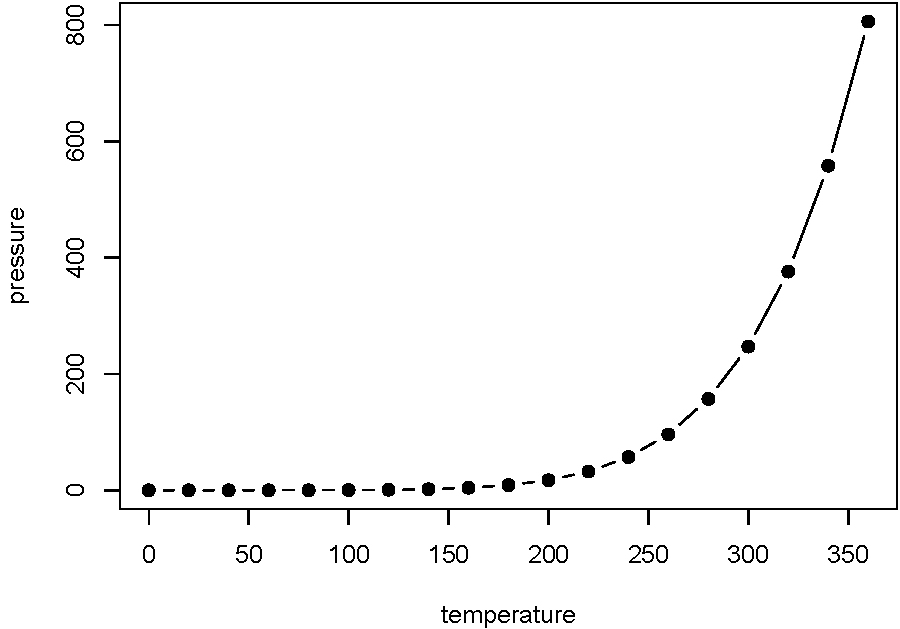
\includegraphics[width=0.9\linewidth]{article_zh_files/figure-latex/pressure-plot-1} 

}

\caption{A figure example with the specified aspect ratio, width, and alignment.}\label{fig:pressure-plot}
\end{figure}

\texttt{fig.width} 和
\texttt{fig.height}给出的是图形的实际大小。我们可以用 \texttt{out.width}
和 \texttt{out.height} 给出图形的输出大小。例如,
\texttt{out.width\ =\ \textquotesingle{}70\%\textquotesingle{}}
\textbf{knitr} 会自动处理为
\texttt{.7\textbackslash{}linewidth},即文本宽度的70\%

An example of \texttt{out.width\ =\ 70\%} (图\ref{fig:cars-plot})。

\begin{Shaded}
\begin{Highlighting}[]
\KeywordTok{par}\NormalTok{(}\DataTypeTok{mar =} \KeywordTok{c}\NormalTok{(}\DecValTok{4}\NormalTok{, }\DecValTok{4}\NormalTok{, }\FloatTok{.1}\NormalTok{, }\FloatTok{.1}\NormalTok{))}
\KeywordTok{plot}\NormalTok{(cars, }\DataTypeTok{pch =} \DecValTok{19}\NormalTok{)}
\end{Highlighting}
\end{Shaded}

\begin{figure}

{\centering 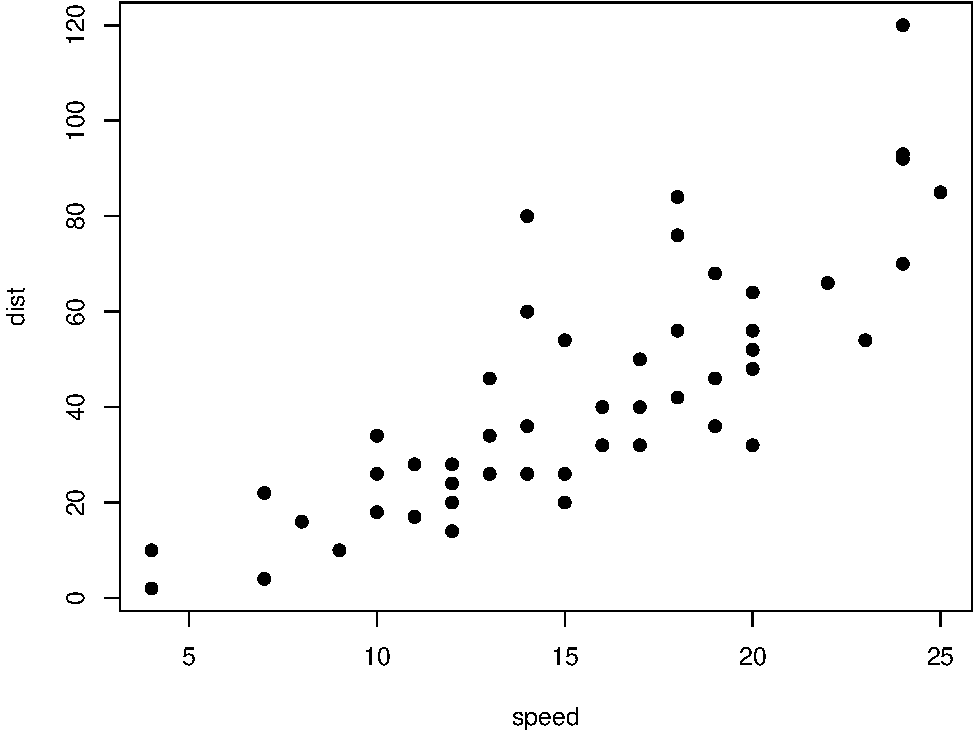
\includegraphics[width=0.7\linewidth]{article_zh_files/figure-latex/cars-plot-1} 

}

\caption{A figure example with a relative width 70\%.}\label{fig:cars-plot}
\end{figure}

如果一幅图里有多个子图,必须设
\texttt{fig.show\ =\ \textquotesingle{}hold\textquotesingle{}},并排图形加起来宽度不能超过文本宽度。如两个子图并排,每个不能超过\texttt{50\%}。

An example of two plots, each with a width of \texttt{45\%}
(图\ref{fig:multi-plots})。

\begin{Shaded}
\begin{Highlighting}[]
\KeywordTok{par}\NormalTok{(}\DataTypeTok{mar =} \KeywordTok{c}\NormalTok{(}\DecValTok{4}\NormalTok{, }\DecValTok{4}\NormalTok{, }\FloatTok{.1}\NormalTok{, }\FloatTok{.1}\NormalTok{))}
\KeywordTok{plot}\NormalTok{(pressure, }\DataTypeTok{pch =} \DecValTok{19}\NormalTok{, }\DataTypeTok{type =} \StringTok{'b'}\NormalTok{)}
\KeywordTok{plot}\NormalTok{(cars, }\DataTypeTok{pch =} \DecValTok{19}\NormalTok{)}
\end{Highlighting}
\end{Shaded}

\begin{figure}

{\centering 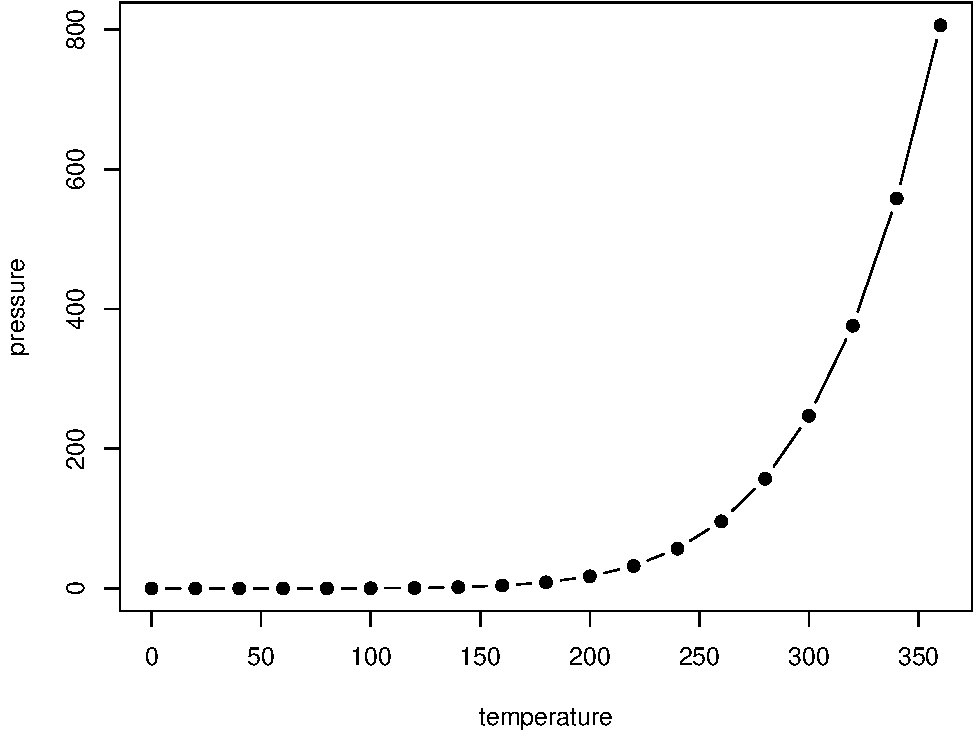
\includegraphics[width=0.45\linewidth]{article_zh_files/figure-latex/multi-plots-1} 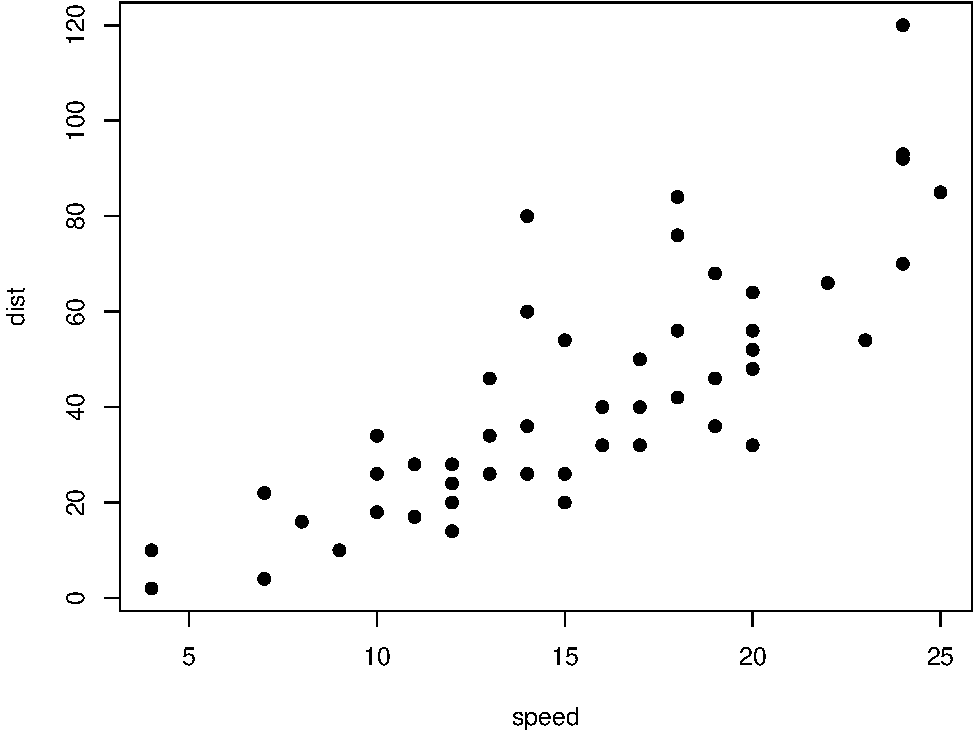
\includegraphics[width=0.45\linewidth]{article_zh_files/figure-latex/multi-plots-2} 

}

\caption{Two plots placed side by side.}\label{fig:multi-plots}
\end{figure}

\subsubsection{插入图形}

R Markdown 用函数 \texttt{knitr::include\_graphics()}
插入图形,要指明图形文件路径(图\ref{fig:run})。

\begin{Shaded}
\begin{Highlighting}[]
\NormalTok{knitr}\OperatorTok{::}\KeywordTok{include_graphics}\NormalTok{(}\StringTok{'images/run.jpg'}\NormalTok{)}
\end{Highlighting}
\end{Shaded}

\begin{figure}

{\centering 
\includegraphics[width=0.5\linewidth]{images/run} 

}

\caption{image included in the document from an external PNG file.}\label{fig:run}
\end{figure}

插入图片可以用 \texttt{include\_graphics()} ,也可以用 Markdown 的
\texttt{!{[}{]}()}。

\textbf{用 \texttt{include\_graphics()} 插入图形有几大优点}:

\begin{enumerate}
\def\labelenumi{\arabic{enumi}.}
\tightlist
\item
  You do not need to worry about the document output format, e.g., when
  the output format is LaTeX, you may have to use the LaTeX command
  \texttt{\textbackslash{}includegraphics\{\}} to include an image, and
  when the output format is Markdown, you have to use
  \texttt{!{[}{]}()}. The function \texttt{include\_graphics()} in
  \textbf{knitr} takes care of these details automatically.
\item
  The syntax for controlling the image attributes is the same as when
  images are generated from R code, e.g., chunk options
  \texttt{fig.cap}, \texttt{out.width}, and \texttt{fig.show} still have
  the same meanings.
\item
  \texttt{include\_graphics()} can be smart enough to use PDF graphics
  automatically when the output format is LaTeX and the PDF graphics
  files exist, e.g., an image path \texttt{foo/bar.png} can be
  automatically replaced with \texttt{foo/bar.pdf} if the latter exists.
  PDF images often have better qualities than raster images in LaTeX/PDF
  output. To make use of this feature, set the argument
  \texttt{auto\_pdf\ =\ TRUE}, or set the global option
  \texttt{options(knitr.graphics.auto\_pdf\ =\ TRUE)} to enable this
  feature globally in an R session.
\item
  You can easily scale these images proportionally using the same ratio.
  This can be done via the \texttt{dpi} argument (dots per inch), which
  takes the value from the chunk option \texttt{dpi} by default. If it
  is a numeric value and the chunk option \texttt{out.width} is not set,
  the output width of an image will be its actual width (in pixels)
  divided by \texttt{dpi}, and the unit will be inches. For example, for
  an image with the size 672 x 480, its output width will be 7 inches
  (\texttt{7in}) when \texttt{dpi\ =\ 96}. This feature requires the
  package \textbf{png} and/or \textbf{jpeg} to be installed. You can
  always override the automatic calculation of width in inches by
  providing a non-NULL value to the chunk option \texttt{out.width}, or
  use \texttt{include\_graphics(dpi\ =\ NA)}.
\end{enumerate}

\subsection{交叉引用}

Rmarkdown没有交叉引用(cross-reference)功能,但是bookdown可以。
交叉引用包括数学公式、定理、图形、表格和章节。

用法:

\begin{itemize}
\item
  标记: 公式\texttt{(\textbackslash{}\#eq:label)},图形
  \texttt{(\textbackslash{}\#fig:label)},表格
  \texttt{(\textbackslash{}\#tab:label)},章节\texttt{\{\#label\}}等。
\item
  引用:\texttt{\textbackslash{}@ref(eq:label)},\texttt{\textbackslash{}@ref(fig:label)},\texttt{\textbackslash{}@ref(tab:label)},
  章节 \texttt{\textbackslash{}@ref(label)}。
\end{itemize}

\hypertarget{equations}{%
\subsubsection{数学公式}\label{equations}}

要给公式编号,先要建立公式环境,然后标记
\texttt{(\textbackslash{}\#eq:label)},例如

\begin{Shaded}
\begin{Highlighting}[]
\KeywordTok{\textbackslash{}begin}\NormalTok{\{}\ExtensionTok{equation}\NormalTok{\}}\SpecialStringTok{ }
\SpecialStringTok{  f}\SpecialCharTok{\textbackslash{}left}\SpecialStringTok{(k}\SpecialCharTok{\textbackslash{}right}\SpecialStringTok{) = }\SpecialCharTok{\textbackslash{}binom}\SpecialStringTok{\{n\}\{k\} p^k}\SpecialCharTok{\textbackslash{}left}\SpecialStringTok{(1-p}\SpecialCharTok{\textbackslash{}right}\SpecialStringTok{)^\{n-k\}}
\SpecialStringTok{  (}\SpecialCharTok{\textbackslash{}#}\SpecialStringTok{eq:binom)}
\KeywordTok{\textbackslash{}end}\NormalTok{\{}\ExtensionTok{equation}\NormalTok{\} }
\end{Highlighting}
\end{Shaded}

结果如下:

\begin{equation}
f\left(k\right)=\binom{n}{k}p^k\left(1-p\right)^{n-k} \label{eq:binom}
\end{equation}

你可以用\texttt{\textbackslash{}@ref(eq:binom)}引用,如,参看公式
\eqref{eq:binom}。

如果公式不需要自动编号,可建立 \texttt{equation*}环境:

\begin{Shaded}
\begin{Highlighting}[]
\KeywordTok{\textbackslash{}begin}\NormalTok{\{}\ExtensionTok{equation*}\NormalTok{\}}\SpecialStringTok{ }
\SpecialCharTok{\textbackslash{}frac}\SpecialStringTok{\{d\}\{dx\}}\SpecialCharTok{\textbackslash{}left}\SpecialStringTok{( }\SpecialCharTok{\textbackslash{}int}\SpecialStringTok{_\{a\}^\{x\} f(u)}\SpecialCharTok{\textbackslash{},}\SpecialStringTok{du}\SpecialCharTok{\textbackslash{}right}\SpecialStringTok{)=f(x)}
\KeywordTok{\textbackslash{}end}\NormalTok{\{}\ExtensionTok{equation*}\NormalTok{\} }
\end{Highlighting}
\end{Shaded}

\begin{equation*}
\frac{d}{dx}\left( \int_{a}^{x} f(u)\,du\right)=f(x)
\end{equation*}

公式对齐:用
\texttt{align},\texttt{=}号左侧加上对齐标记\texttt{\&};换行用
\texttt{\textbackslash{}\textbackslash{}}。默认情况下,\texttt{align}
环境里每行都会指定一个编号,如果某行不要编号,可用
\texttt{\textbackslash{}notag}。

\begin{Shaded}
\begin{Highlighting}[]
\KeywordTok{\textbackslash{}begin}\NormalTok{\{}\ExtensionTok{align}\NormalTok{\}}\SpecialStringTok{ }
\SpecialStringTok{g(X_\{n\}) &= g(}\SpecialCharTok{\textbackslash{}theta}\SpecialStringTok{)+g'(\{}\SpecialCharTok{\textbackslash{}tilde}\SpecialStringTok{\{}\SpecialCharTok{\textbackslash{}theta}\SpecialStringTok{\}\})(X_\{n\}-}\SpecialCharTok{\textbackslash{}theta}\SpecialStringTok{) }\SpecialCharTok{\textbackslash{}notag}\SpecialStringTok{ }\SpecialCharTok{\textbackslash{}\textbackslash{}}
\SpecialCharTok{\textbackslash{}sqrt}\SpecialStringTok{\{n\}[g(X_\{n\})-g(}\SpecialCharTok{\textbackslash{}theta}\SpecialStringTok{)] &= g'}\SpecialCharTok{\textbackslash{}left}\SpecialStringTok{(\{}\SpecialCharTok{\textbackslash{}tilde}\SpecialStringTok{\{}\SpecialCharTok{\textbackslash{}theta}\SpecialStringTok{\}\}}\SpecialCharTok{\textbackslash{}right}\SpecialStringTok{)}
\SpecialStringTok{  }\SpecialCharTok{\textbackslash{}sqrt}\SpecialStringTok{\{n\}[X_\{n\}-}\SpecialCharTok{\textbackslash{}theta}\SpecialStringTok{ ] (}\SpecialCharTok{\textbackslash{}#}\SpecialStringTok{eq:align)}
\KeywordTok{\textbackslash{}end}\NormalTok{\{}\ExtensionTok{align}\NormalTok{\} }
\end{Highlighting}
\end{Shaded}

\begin{align}
g(X_{n}) &= g(\theta)+g'({\tilde{\theta}})(X_{n}-\theta) \notag \\
\sqrt{n}[g(X_{n})-g(\theta)] &= g'\left({\tilde{\theta}}\right)
  \sqrt{n}[X_{n}-\theta ] \label{eq:align}
\end{align}

如果一个公式有多行,希望共享一个编号,可用 \texttt{split}环境:

\begin{Shaded}
\begin{Highlighting}[]
\KeywordTok{\textbackslash{}begin}\NormalTok{\{}\ExtensionTok{equation}\NormalTok{\}}\SpecialStringTok{ }
\KeywordTok{\textbackslash{}begin}\NormalTok{\{}\ExtensionTok{split}\NormalTok{\}}
\SpecialCharTok{\textbackslash{}mathrm}\SpecialStringTok{\{Var\}(}\SpecialCharTok{\textbackslash{}hat}\SpecialStringTok{\{}\SpecialCharTok{\textbackslash{}beta}\SpecialStringTok{\}) & =}\SpecialCharTok{\textbackslash{}mathrm}\SpecialStringTok{\{Var\}((X'X)^\{-1\}X'y)}\SpecialCharTok{\textbackslash{}\textbackslash{}}
\SpecialStringTok{ & =(X'X)^\{-1\}X'}\SpecialCharTok{\textbackslash{}mathrm}\SpecialStringTok{\{Var\}(y)((X'X)^\{-1\}X')'}\SpecialCharTok{\textbackslash{}\textbackslash{}}
\SpecialStringTok{ & =(X'X)^\{-1\}X'}\SpecialCharTok{\textbackslash{}mathrm}\SpecialStringTok{\{Var\}(y)X(X'X)^\{-1\}}\SpecialCharTok{\textbackslash{}\textbackslash{}}
\SpecialStringTok{ & =(X'X)^\{-1\}X'}\SpecialCharTok{\textbackslash{}sigma}\SpecialStringTok{^\{2\}IX(X'X)^\{-1\}}\SpecialCharTok{\textbackslash{}\textbackslash{}}
\SpecialStringTok{ & =(X'X)^\{-1\}}\SpecialCharTok{\textbackslash{}sigma}\SpecialStringTok{^\{2\}}
\KeywordTok{\textbackslash{}end}\NormalTok{\{}\SpecialStringTok{split\}}
\SpecialStringTok{(}\SpecialCharTok{\textbackslash{}#}\SpecialStringTok{eq:var-beta)}
\KeywordTok{\textbackslash{}end}\NormalTok{\{}\ExtensionTok{equation}\NormalTok{\} }
\end{Highlighting}
\end{Shaded}

\begin{equation}
\begin{split}
\mathrm{Var}(\hat{\beta}) & =\mathrm{Var}((X'X)^{-1}X'y)\\
 & =(X'X)^{-1}X'\mathrm{Var}(y)((X'X)^{-1}X')'\\
 & =(X'X)^{-1}X'\mathrm{Var}(y)X(X'X)^{-1}\\
 & =(X'X)^{-1}X'\sigma^{2}IX(X'X)^{-1}\\
 & =(X'X)^{-1}\sigma^{2}
\end{split}
\label{eq:var-beta}
\end{equation}

\hypertarget{theorems}{%
\subsubsection{定理}\label{theorems}}

用下面形式创建一个定理环境:

\begin{Shaded}
\begin{Highlighting}[]
\NormalTok{```\{theorem,label="yourlabel",name="theorem name"\}}
\NormalTok{Here is my theorem.}
\NormalTok{```}
\end{Highlighting}
\end{Shaded}

一个定理的例子:

\begin{Shaded}
\begin{Highlighting}[]
\NormalTok{```\{theorem, pyth, name="Pythagorean theorem"\}}
\NormalTok{For a right triangle, if $c$ denotes the length of the hypotenuse}
\NormalTok{and $a$ and $b$ denote the lengths of the other two sides, we have}

\NormalTok{$$a^2 + b^2 = c^2$$}
\NormalTok{```}
\end{Highlighting}
\end{Shaded}

结果如下:

\BeginKnitrBlock{theorem}[Pythagorean theorem]
\protect\hypertarget{thm:pyth}{}{\label{thm:pyth} \iffalse (Pythagorean
theorem) \fi{} }For a right triangle, if \(c\) denotes the length of the
hypotenuse and \(a\) and \(b\) denote the lengths of the other two
sides, we have

\[a^2 + b^2 = c^2\]
\EndKnitrBlock{theorem}

引用用法:在需要引用处插入\texttt{\textbackslash{}@ref(thm:label)}。

参看定理 \ref{thm:pyth}。见定义\ref{def:char}。

定义、推论、命题、公里、假设等类似。

注意,如果 \texttt{echo}设置为\texttt{FALSE},定理编号失效。

\BeginKnitrBlock{definition}
\protect\hypertarget{def:char}{}{\label{def:char} }随机变量 \(X\)
的特征函数定义为
\[\varphi _{X}(t)=\operatorname {E} \left[e^{itX}\right], \; t\in\mathcal{R}\]
\EndKnitrBlock{definition}

\BeginKnitrBlock{example}
\protect\hypertarget{exm:unnamed-chunk-4}{}{\label{exm:unnamed-chunk-4} }We
derive the characteristic function of \(X\sim U(0,1)\) with the
probability density function \(f(x)=\mathbf{1}_{x \in [0,1]}\).

\begin{equation*}
\begin{split}
\varphi _{X}(t) &= \operatorname {E} \left[e^{itX}\right]\\
 & =\int e^{itx}f(x)dx\\
 & =\int_{0}^{1}e^{itx}dx\\
 & =\int_{0}^{1}\left(\cos(tx)+i\sin(tx)\right)dx\\
 & =\left.\left(\frac{\sin(tx)}{t}-i\frac{\cos(tx)}{t}\right)\right|_{0}^{1}\\
 & =\frac{\sin(t)}{t}-i\left(\frac{\cos(t)-1}{t}\right)\\
 & =\frac{i\sin(t)}{it}+\frac{\cos(t)-1}{it}\\
 & =\frac{e^{it}-1}{it}
\end{split}
\end{equation*}

Note that we used the fact \(e^{ix}=\cos(x)+i\sin(x)\) twice.
\EndKnitrBlock{example}

\BeginKnitrBlock{lemma}
\protect\hypertarget{lem:chf-pdf}{}{\label{lem:chf-pdf} }For any two random
variables \(X_1\), \(X_2\), they both have the same probability
distribution if and only if

\[\varphi _{X_1}(t)=\varphi _{X_2}(t)\]
\EndKnitrBlock{lemma}

\BeginKnitrBlock{theorem}
\protect\hypertarget{thm:chf-sum}{}{\label{thm:chf-sum} }If \(X_1\),
\ldots{}, \(X_n\) are independent random variables, and \(a_1\),
\ldots{}, \(a_n\) are some constants, then the characteristic function
of the linear combination \(S_n=\sum_{i=1}^na_iX_i\) is

\[\varphi _{S_{n}}(t)=\prod_{i=1}^n\varphi _{X_i}(a_{i}t)=\varphi _{X_{1}}(a_{1}t)\cdots \varphi _{X_{n}}(a_{n}t)\]
\EndKnitrBlock{theorem}

\BeginKnitrBlock{proposition}
\protect\hypertarget{prp:unnamed-chunk-5}{}{\label{prp:unnamed-chunk-5} }The
distribution of the sum of independent Poisson random variables
\(X_i \sim \mathrm{Pois}(\lambda_i),\: i=1,2,\cdots,n\) is
\(\mathrm{Pois}(\sum_{i=1}^n\lambda_i)\).
\EndKnitrBlock{proposition}

This is the characteristic function of a Poisson random variable with
the parameter \(\lambda=\sum_{i=1}^n \lambda_i\). From Lemma
\ref{lem:chf-pdf}, we know the distribution of \(P_n\) is
\(\mathrm{Pois}(\sum_{i=1}^n\lambda_i)\).

\BeginKnitrBlock{remark}
\iffalse{} {Remark. } \fi{}In some cases, it is very convenient and easy
to figure out the distribution of the sum of independent random
variables using characteristic functions.
\EndKnitrBlock{remark}

\BeginKnitrBlock{corollary}
\protect\hypertarget{cor:unnamed-chunk-7}{}{\label{cor:unnamed-chunk-7} }The
characteristic function of the sum of two independent random variables
\(X_1\) and \(X_2\) is the product of characteristic functions of
\(X_1\) and \(X_2\), i.e.,
\[\varphi _{X_1+X_2}(t)=\varphi _{X_1}(t) \varphi _{X_2}(t)\]
\EndKnitrBlock{corollary}

\hypertarget{ggplot2}{%
\subsection{一个ggplot2作图的例子}\label{ggplot2}}

\texttt{ggplot2}的几个基本概念:

\begin{itemize}
\tightlist
\item
  数据(Data)和映射(Mapping):将数据映到图像
\item
  几何对象(Geometric):代表在图中看到的实际元素,如点、线、多边形等
\item
  统计变换(Statistics):对数据进行某种汇总,如直方图,或将二维关系用线性模型解释
\item
  标度(Scale):将数据的取值映射到图形空间,例如用:颜色、大小、形状表示不同取值
\item
  坐标系(Coordinate):数据如何映射到图形所在平面,提供作图所需的坐标轴和网格线
\item
  分面(Facet):将数据分解为子集,进行联合展示
\item
  图层(Layer):对所需的绘图操作进行一层一层叠加,最终得到所需图形
\end{itemize}

\subsubsection{散点图}

\begin{Shaded}
\begin{Highlighting}[]
\KeywordTok{library}\NormalTok{(ggplot2)}
\NormalTok{p <-}\StringTok{ }\KeywordTok{ggplot}\NormalTok{(}\DataTypeTok{data =}\NormalTok{ mpg, }\DataTypeTok{mapping =} \KeywordTok{aes}\NormalTok{(}\DataTypeTok{x =}\NormalTok{ cty, }\DataTypeTok{y =}\NormalTok{ hwy))}
\NormalTok{p }\OperatorTok{+}\StringTok{ }\KeywordTok{geom_point}\NormalTok{()}
\end{Highlighting}
\end{Shaded}

\begin{figure}

{\centering 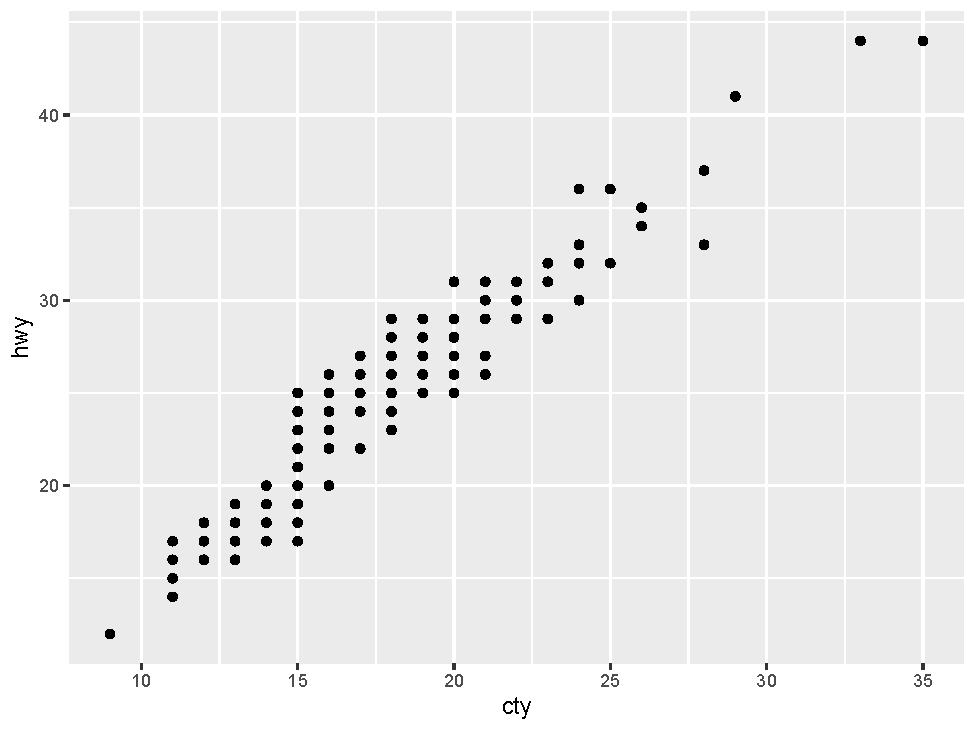
\includegraphics[width=0.75\linewidth]{article_zh_files/figure-latex/points-1} 

}

\caption{ggplot2 with points}\label{fig:points}
\end{figure}

第一行指定数据集、映射(坐标轴),第二行表示在\texttt{p}的基础上加上点,\texttt{geom}表示的是
geometric object(几何对象)(见图\ref{fig:points})。

mpg是ggplot2里面的一个关于汽车的数据集。

\begin{itemize}
\tightlist
\item
  cty:city miles per gallon
\item
  hwy:highway miles per gallon
\item
  year:year of manufacture
\item
  displ:engine displacement, in litres
\item
  cyl:number of cylinders
\item
  class:``type'' of car
\end{itemize}

\subsubsection{变换颜色}

按生产年份以颜色区分,\texttt{factor(year))}是把年份转化为因子形式(相当于定类变量),
见图 \ref{fig:colors}。

\begin{Shaded}
\begin{Highlighting}[]
\NormalTok{p <-}\StringTok{ }\KeywordTok{ggplot}\NormalTok{(mpg, }\KeywordTok{aes}\NormalTok{(}\DataTypeTok{x =}\NormalTok{ cty, }\DataTypeTok{y =}\NormalTok{ hwy, }\DataTypeTok{colour =} \KeywordTok{factor}\NormalTok{(year)))}
\NormalTok{p }\OperatorTok{+}\StringTok{ }\KeywordTok{geom_point}\NormalTok{()}
\end{Highlighting}
\end{Shaded}

\begin{figure}

{\centering 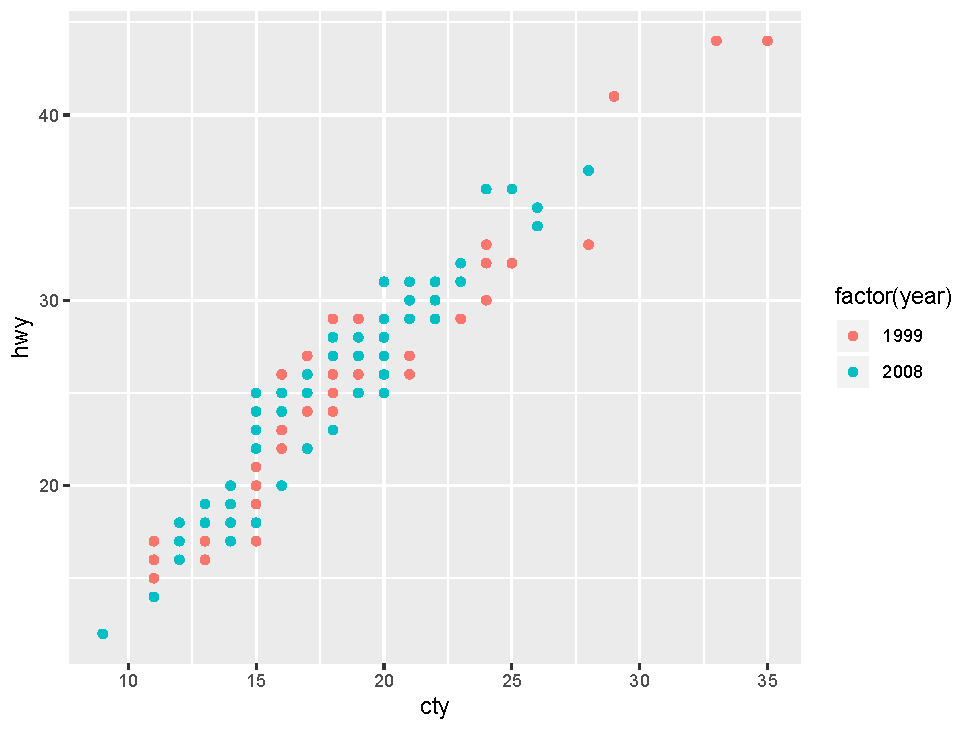
\includegraphics[width=0.75\linewidth]{article_zh_files/figure-latex/colors-1} 

}

\caption{ggplot2 with points colors}\label{fig:colors}
\end{figure}

\subsubsection{拟合曲线}

再加一行 \texttt{+\ stat\_smooth()},其中\texttt{stat}表示 statistical
transformation,做了统计平滑拟合直线,以及置信区间, 见图
\ref{fig:trends}。

\begin{Shaded}
\begin{Highlighting}[]
\NormalTok{p }\OperatorTok{+}\StringTok{ }\KeywordTok{geom_point}\NormalTok{() }\OperatorTok{+}\StringTok{ }\KeywordTok{stat_smooth}\NormalTok{()}
\end{Highlighting}
\end{Shaded}

\begin{figure}

{\centering 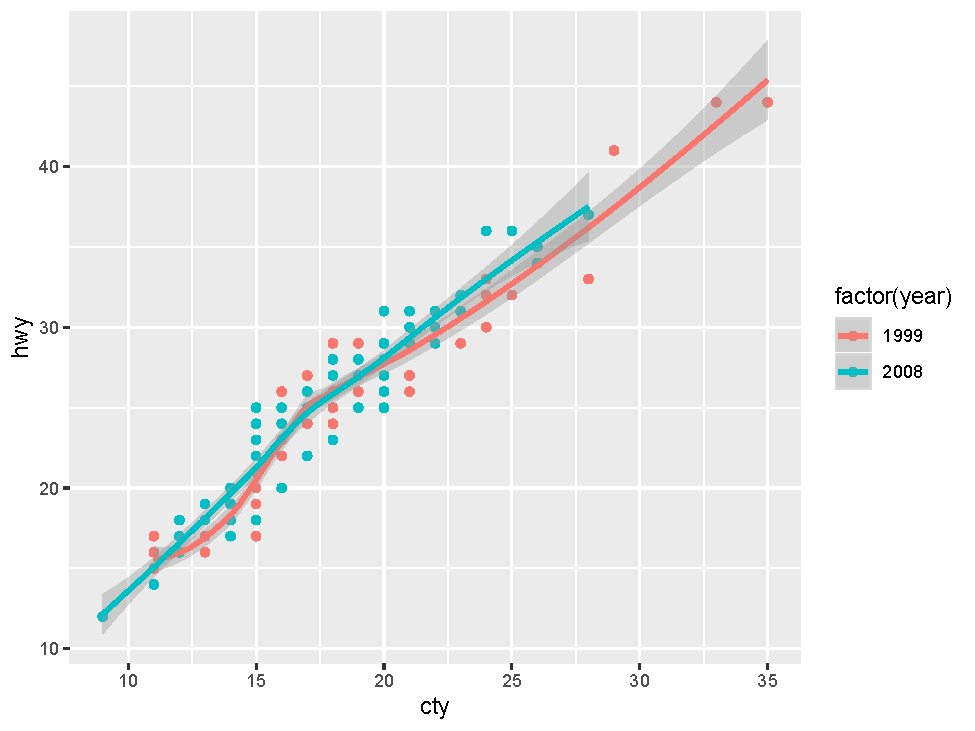
\includegraphics[width=0.75\linewidth]{article_zh_files/figure-latex/trends-1} 

}

\caption{ggplot2 with smooth trends}\label{fig:trends}
\end{figure}

\subsubsection{变换大小}

上图的数据点明显偏小,可以让这些数据点随着\textbf{汽车排量}的大小而变化,
见图 \ref{fig:size}。

\begin{Shaded}
\begin{Highlighting}[]
\NormalTok{p }\OperatorTok{+}\StringTok{ }\KeywordTok{geom_point}\NormalTok{(}\KeywordTok{aes}\NormalTok{(}\DataTypeTok{colour =} \KeywordTok{factor}\NormalTok{(year), }\DataTypeTok{size =}\NormalTok{ displ)) }\OperatorTok{+}\StringTok{ }
\StringTok{  }\KeywordTok{stat_smooth}\NormalTok{()   }\CommentTok{# 排量越大,点越大}
\end{Highlighting}
\end{Shaded}

\begin{figure}

{\centering 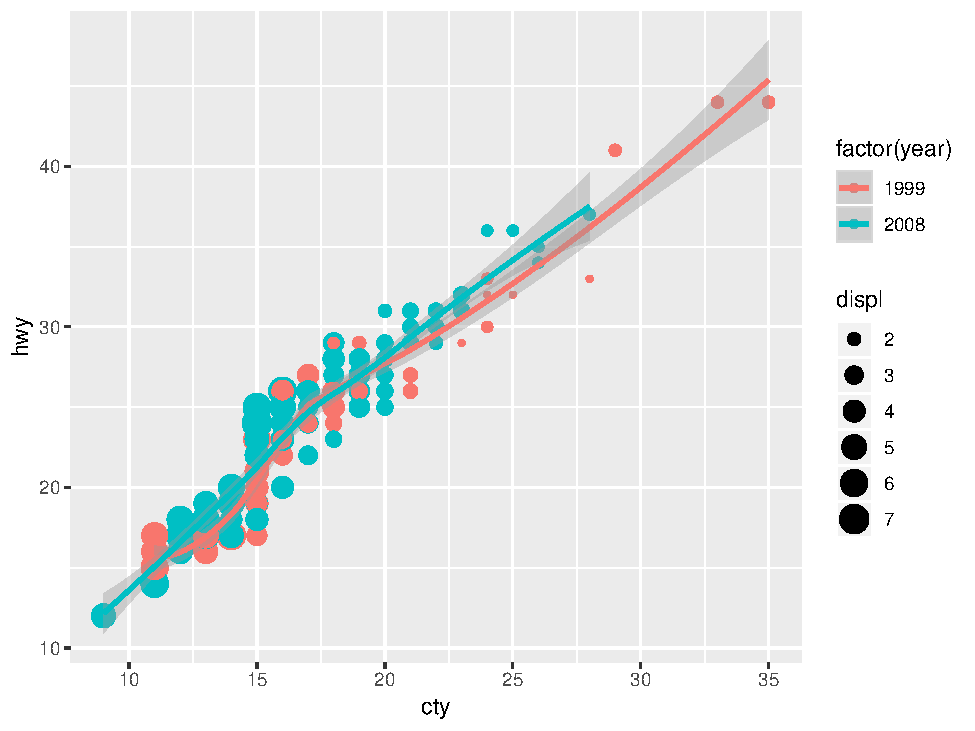
\includegraphics[width=0.75\linewidth]{article_zh_files/figure-latex/size-1} 

}

\caption{ggplot2 with variable point size}\label{fig:size}
\end{figure}

\subsubsection{修改透明度}

数据点太密集,增加透明度,解决点与点之间的重叠的问题, 见图
\ref{fig:trans}。

\begin{Shaded}
\begin{Highlighting}[]
\NormalTok{p }\OperatorTok{+}\StringTok{ }\KeywordTok{geom_point}\NormalTok{(}\KeywordTok{aes}\NormalTok{(}\DataTypeTok{colour =} \KeywordTok{factor}\NormalTok{(year),}
                   \DataTypeTok{size =}\NormalTok{ displ), }\DataTypeTok{alpha =} \FloatTok{0.5}\NormalTok{) }\OperatorTok{+}
\StringTok{  }\KeywordTok{stat_smooth}\NormalTok{() }\OperatorTok{+}\StringTok{ }\KeywordTok{scale_size_continuous}\NormalTok{(}\DataTypeTok{range =} \KeywordTok{c}\NormalTok{(}\DecValTok{4}\NormalTok{, }\DecValTok{10}\NormalTok{))}
\end{Highlighting}
\end{Shaded}

\begin{figure}

{\centering 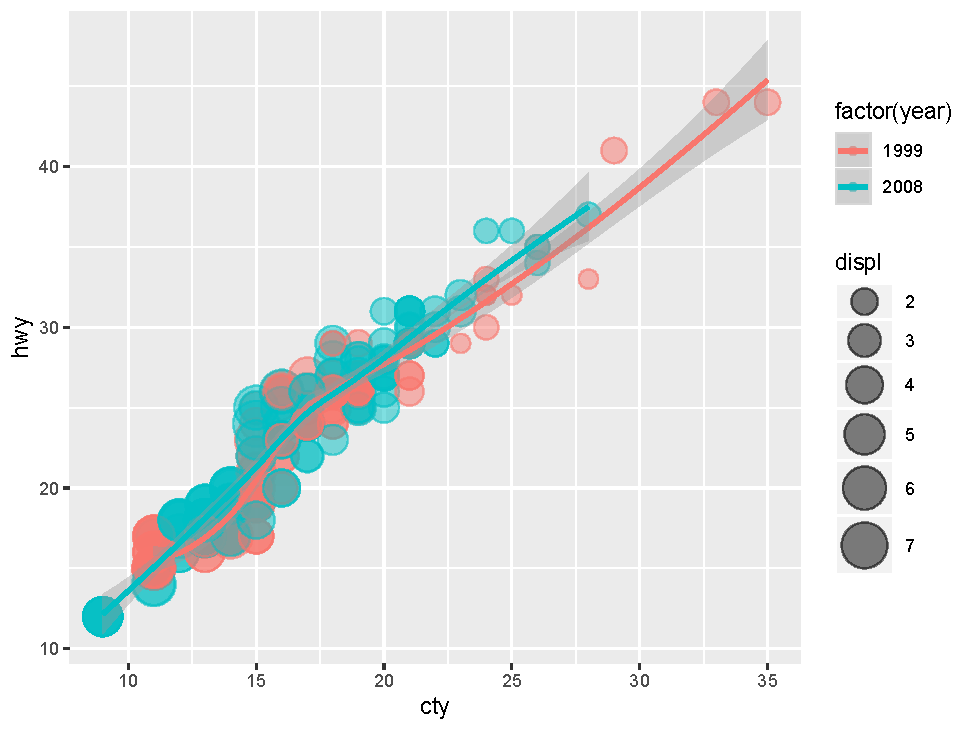
\includegraphics[width=0.75\linewidth]{article_zh_files/figure-latex/trans-1} 

}

\caption{ggplot2 with transparent points}\label{fig:trans}
\end{figure}

\texttt{alpha=0.5}
在\texttt{aes()}的外面,代表对所有的点都强制透明度为0.5。

\subsubsection{图形分层}

1999年与2008年数据点全部挤在一块,太拥挤了,应采用分层,见图
\ref{fig:facet}。

\begin{Shaded}
\begin{Highlighting}[]
\NormalTok{p }\OperatorTok{+}\StringTok{ }\KeywordTok{geom_point}\NormalTok{(}\KeywordTok{aes}\NormalTok{(}\DataTypeTok{colour =}\NormalTok{ class, }\DataTypeTok{size =}\NormalTok{ displ), }\DataTypeTok{alpha =} \FloatTok{0.5}\NormalTok{) }\OperatorTok{+}
\StringTok{  }\KeywordTok{stat_smooth}\NormalTok{() }\OperatorTok{+}\StringTok{ }\KeywordTok{scale_size_continuous}\NormalTok{(}\DataTypeTok{range =} \KeywordTok{c}\NormalTok{(}\DecValTok{4}\NormalTok{, }\DecValTok{10}\NormalTok{)) }\OperatorTok{+}
\StringTok{  }\KeywordTok{facet_wrap}\NormalTok{(}\OperatorTok{~}\StringTok{ }\NormalTok{year, }\DataTypeTok{ncol =} \DecValTok{1}\NormalTok{)}
\end{Highlighting}
\end{Shaded}

\begin{figure}

{\centering 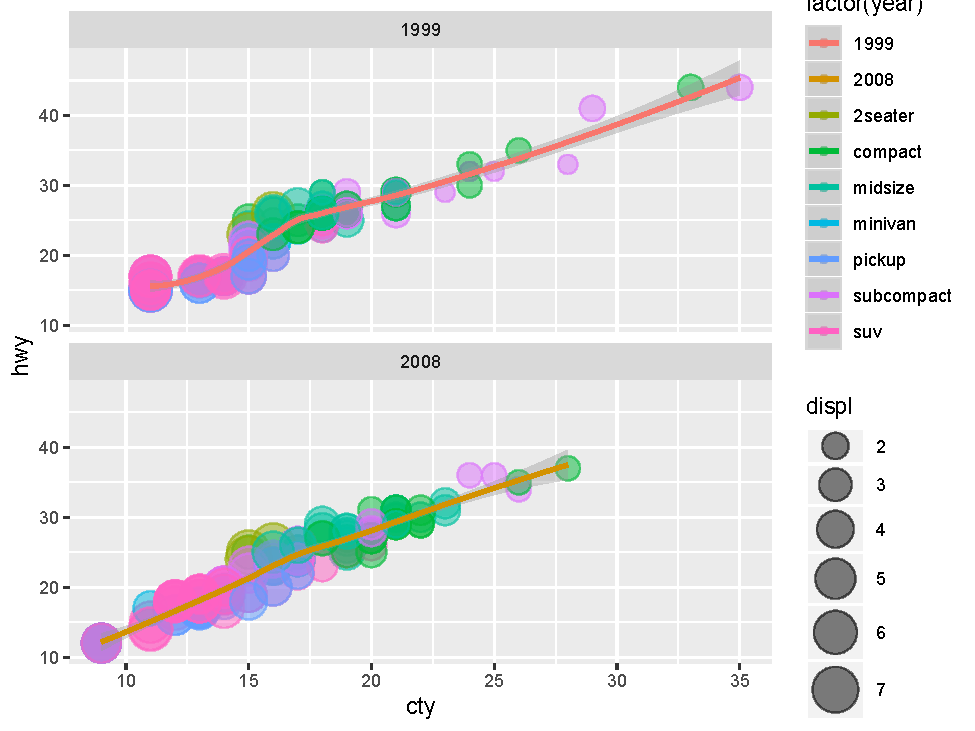
\includegraphics[width=0.75\linewidth]{article_zh_files/figure-latex/facet-1} 

}

\caption{ggplot2 with facets}\label{fig:facet}
\end{figure}

\begin{itemize}
\tightlist
\item
  \texttt{facet\_wrap()}
  是\texttt{facet}与\texttt{wrap}两个词组合,表示逐面包起来。
\item
  \texttt{\textasciitilde{}year}
  表示按变量\texttt{year}分层,将1999与2008分开。
\item
  \texttt{ncol\ =\ 1}
  代表小窗口是1列,指定了1列之后,默认就是两行(因为年份一共只有两种)。如果不加这句,会默认横着排列,或者想要指定几行,则使用\texttt{nrow\ =\ 1}。
\item
  这里颜色指定了 \texttt{colour\ =\ class},代表不同种类的汽车。
\item
  添加了\texttt{scale\_size\_continuous(range\ =\ c(4,\ 10))},指定\texttt{size}的变化范围。在本图中,就是控制点的绝对大小的范围,
  不要太大,也不要太小。
\end{itemize}

\subsubsection{添加中文标注}

默认情况下图形上是不能出现中文的,要使得中文在图形中正常显示,必须在文档开头的\texttt{output}下面加上:
\texttt{dev:\ "cairo\_pdf"}。也可以在作图时加上\texttt{pdf.options(family="GB1")}。

\begin{Shaded}
\begin{Highlighting}[]
\NormalTok{p }\OperatorTok{+}\StringTok{ }\KeywordTok{geom_point}\NormalTok{(}\KeywordTok{aes}\NormalTok{(}\DataTypeTok{colour =}\NormalTok{ class, }\DataTypeTok{size =}\NormalTok{ displ), }\DataTypeTok{alpha=}\FloatTok{0.5}\NormalTok{) }\OperatorTok{+}
\StringTok{  }\KeywordTok{stat_smooth}\NormalTok{() }\OperatorTok{+}\StringTok{ }\KeywordTok{scale_size_continuous}\NormalTok{(}\DataTypeTok{range =} \KeywordTok{c}\NormalTok{(}\DecValTok{4}\NormalTok{, }\DecValTok{10}\NormalTok{)) }\OperatorTok{+}
\StringTok{  }\KeywordTok{facet_wrap}\NormalTok{(}\OperatorTok{~}\StringTok{ }\NormalTok{year,}\DataTypeTok{ncol =} \DecValTok{1}\NormalTok{) }\OperatorTok{+}
\StringTok{  }\KeywordTok{labs}\NormalTok{(}\DataTypeTok{y =} \StringTok{'每加仑高速公路行驶距离'}\NormalTok{, }\DataTypeTok{x =} \StringTok{'每加仑城市公路行驶距离'}\NormalTok{,}
       \DataTypeTok{title =} \StringTok{'汽车油耗与型号'}\NormalTok{, }\DataTypeTok{size =} \StringTok{'排量'}\NormalTok{, }\DataTypeTok{colour =} \StringTok{'车型'}\NormalTok{) }\OperatorTok{+}
\StringTok{  }\KeywordTok{theme}\NormalTok{(}\DataTypeTok{text =} \KeywordTok{element_text}\NormalTok{(}\DataTypeTok{family =} \StringTok{"STHeiti"}\NormalTok{),}
        \DataTypeTok{plot.title =} \KeywordTok{element_text}\NormalTok{(}\DataTypeTok{hjust =} \FloatTok{0.5}\NormalTok{))}
\end{Highlighting}
\end{Shaded}

\begin{figure}

{\centering 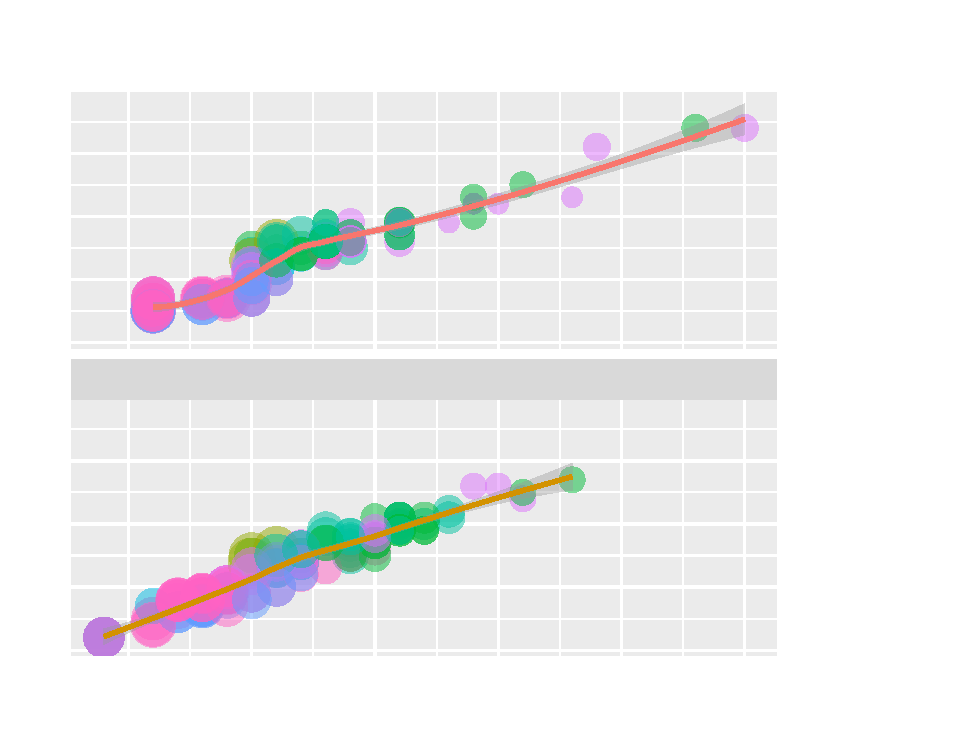
\includegraphics[width=0.75\linewidth]{article_zh_files/figure-latex/zh-1} 

}

\caption{ggplot2 with Chinese characters}\label{fig:zh}
\end{figure}

图 \ref{fig:zh}中,

\begin{itemize}
\tightlist
\item
  \texttt{labs()}修改的是标签的名称。
\item
  \texttt{theme()}主题,更偏向于格式的修改。\texttt{text\ =\ element\_text(family\ =\ "STHeiti")}
  是对字体进行修改,变为黑体。Windows系统可以不添加这行,一样会显示前面labs()中设定的中文。而如果是Mac或者Linux系统,由于字体的缺失,会显示成一个一个的框框,在图像上显示不了中文字。
\item
  \texttt{plot.title\ =\ element\_text(hjust\ =\ 0.5)}
  调整标题的位置,不加这行,标题会居左,加上才会居中。\texttt{hjust\ =\ 0.5}
  其实就是左右移动的意思,0.5表示居中。
\end{itemize}

这个例子来自
\url{https://blog.csdn.net/weixin_41929524/article/details/79765882}。

\subsection{表格}

\hypertarget{rkable}{%
\subsubsection{\texorpdfstring{用R函数\texttt{kable()}制作表格}{用R函数kable()制作表格}}\label{rkable}}

R Markdown 对数据制作表格最方便的函数是 \texttt{knitr::kable()}。

\begin{Shaded}
\begin{Highlighting}[]
\NormalTok{knitr}\OperatorTok{::}\KeywordTok{kable}\NormalTok{(}
  \KeywordTok{head}\NormalTok{(mtcars[, }\DecValTok{1}\OperatorTok{:}\DecValTok{8}\NormalTok{], }\DecValTok{10}\NormalTok{), }\DataTypeTok{booktabs =} \OtherTok{TRUE}\NormalTok{,}
  \DataTypeTok{caption =} \StringTok{'A table of the first 10 rows of the mtcars data.'}
\NormalTok{)}
\end{Highlighting}
\end{Shaded}

\begin{table}

\caption{\label{tab:table-single}A table of the first 10 rows of the mtcars data.}
\centering
\begin{tabular}[t]{lrrrrrrrr}
\toprule
  & mpg & cyl & disp & hp & drat & wt & qsec & vs\\
\midrule
Mazda RX4 & 21.0 & 6 & 160.0 & 110 & 3.90 & 2.620 & 16.46 & 0\\
Mazda RX4 Wag & 21.0 & 6 & 160.0 & 110 & 3.90 & 2.875 & 17.02 & 0\\
Datsun 710 & 22.8 & 4 & 108.0 & 93 & 3.85 & 2.320 & 18.61 & 1\\
Hornet 4 Drive & 21.4 & 6 & 258.0 & 110 & 3.08 & 3.215 & 19.44 & 1\\
Hornet Sportabout & 18.7 & 8 & 360.0 & 175 & 3.15 & 3.440 & 17.02 & 0\\
\addlinespace
Valiant & 18.1 & 6 & 225.0 & 105 & 2.76 & 3.460 & 20.22 & 1\\
Duster 360 & 14.3 & 8 & 360.0 & 245 & 3.21 & 3.570 & 15.84 & 0\\
Merc 240D & 24.4 & 4 & 146.7 & 62 & 3.69 & 3.190 & 20.00 & 1\\
Merc 230 & 22.8 & 4 & 140.8 & 95 & 3.92 & 3.150 & 22.90 & 1\\
Merc 280 & 19.2 & 6 & 167.6 & 123 & 3.92 & 3.440 & 18.30 & 1\\
\bottomrule
\end{tabular}
\end{table}

If you want to put multiple tables in a single table environment, wrap
the data objects (usually data frames in R) into a list. Please note
that this feature is only available in HTML and PDF output.

\begin{Shaded}
\begin{Highlighting}[]
\NormalTok{knitr}\OperatorTok{::}\KeywordTok{kable}\NormalTok{(}
  \KeywordTok{list}\NormalTok{(}
    \KeywordTok{head}\NormalTok{(iris[, }\DecValTok{1}\OperatorTok{:}\DecValTok{2}\NormalTok{], }\DecValTok{3}\NormalTok{),}
    \KeywordTok{head}\NormalTok{(mtcars[, }\DecValTok{1}\OperatorTok{:}\DecValTok{3}\NormalTok{], }\DecValTok{5}\NormalTok{)}
\NormalTok{  ),}
  \DataTypeTok{caption =} \StringTok{'A Tale of Two Tables.'}\NormalTok{, }\DataTypeTok{booktabs =} \OtherTok{TRUE}
\NormalTok{)}
\end{Highlighting}
\end{Shaded}

\begin{table}
\caption{\label{tab:table-multi}A Tale of Two Tables.}

\centering
\begin{tabular}[t]{rr}
\toprule
Sepal.Length & Sepal.Width\\
\midrule
5.1 & 3.5\\
4.9 & 3.0\\
4.7 & 3.2\\
\bottomrule
\end{tabular}
\centering
\begin{tabular}[t]{lrrr}
\toprule
  & mpg & cyl & disp\\
\midrule
Mazda RX4 & 21.0 & 6 & 160\\
Mazda RX4 Wag & 21.0 & 6 & 160\\
Datsun 710 & 22.8 & 4 & 108\\
Hornet 4 Drive & 21.4 & 6 & 258\\
Hornet Sportabout & 18.7 & 8 & 360\\
\bottomrule
\end{tabular}
\end{table}

在LaTex的pdf中,插图经常会浮动位置。When you do not want a table to
float in PDF, you may use the LaTeX package
\href{https://www.ctan.org/pkg/longtable}{\textbf{longtable},} which can
break a table across multiple pages. To use \textbf{longtable}, pass
\texttt{longtable\ =\ TRUE} to \texttt{kable()}, and make sure to
include \texttt{\textbackslash{}usepackage\{longtable\}} in the LaTeX
preamble for how to customize the LaTeX preamble). Of course, this is
irrelevant to HTML output, since tables in HTML do not need to float.

\begin{Shaded}
\begin{Highlighting}[]
\NormalTok{knitr}\OperatorTok{::}\KeywordTok{kable}\NormalTok{(}
\NormalTok{  iris[}\DecValTok{1}\OperatorTok{:}\DecValTok{5}\NormalTok{, ], }\DataTypeTok{longtable =} \OtherTok{TRUE}\NormalTok{, }\DataTypeTok{booktabs =} \OtherTok{TRUE}\NormalTok{,}
  \DataTypeTok{caption =} \StringTok{'A table generated by the longtable package.'}
\NormalTok{)}
\end{Highlighting}
\end{Shaded}

\begin{longtable}[t]{rrrrl}
\caption{\label{tab:longtable}A table generated by the longtable package.}\\
\toprule
Sepal.Length & Sepal.Width & Petal.Length & Petal.Width & Species\\
\midrule
5.1 & 3.5 & 1.4 & 0.2 & setosa\\
4.9 & 3.0 & 1.4 & 0.2 & setosa\\
4.7 & 3.2 & 1.3 & 0.2 & setosa\\
4.6 & 3.1 & 1.5 & 0.2 & setosa\\
5.0 & 3.6 & 1.4 & 0.2 & setosa\\
\bottomrule
\end{longtable}

\hypertarget{markdown}{%
\subsubsection{制作Markdown表格}\label{markdown}}

用Markdown制作表格很简单,直接用\texttt{-\/-\/-} 和
\texttt{\textbar{}}分隔即可。

Pandoc supports several types of
\href{http://pandoc.org/MANUAL.html\#tables}{Markdown tables,} such as
simple tables, multiline tables, grid tables, and pipe tables. What
\texttt{knitr::kable()} generates is a simple table like this:

\begin{Shaded}
\begin{Highlighting}[]
\NormalTok{Table: A simple table in Markdown.}

\NormalTok{ First Header | Second Header}
\NormalTok{------------- | -------------}
\NormalTok{Content Cell  | Content Cell}
\NormalTok{Content Cell  | Content Cell}
\end{Highlighting}
\end{Shaded}

\begin{longtable}[]{@{}rrrr@{}}
\caption{A simple table in Markdown.}\tabularnewline
\toprule
Sepal.Length & Sepal.Width & Petal.Length & Petal.Width\tabularnewline
\midrule
\endfirsthead
\toprule
Sepal.Length & Sepal.Width & Petal.Length & Petal.Width\tabularnewline
\midrule
\endhead
5.1 & 3.5 & 1.4 & 0.2\tabularnewline
4.9 & 3.0 & 1.4 & 0.2\tabularnewline
4.7 & 3.2 & 1.3 & 0.2\tabularnewline
4.6 & 3.1 & 1.5 & 0.2\tabularnewline
5.0 & 3.6 & 1.4 & 0.2\tabularnewline
5.4 & 3.9 & 1.7 & 0.4\tabularnewline
\bottomrule
\end{longtable}

You can use any types of Markdown tables in your document.

\subsection{文献引用}

学术论文一般做法是,把所有文献以 \textbf{BibTeX}
格式保存为一个\texttt{.bib}文件,然后在论文中随时插入引用。

\textbf{引用}:如果是作者-年格式,\texttt{@R-rmarkdown}
表示作者姓名(年份),而 \texttt{{[}@R-rmarkdown{]}} 则表示(作者
年份)。

如果是编号格式,则\texttt{@R-rmarkdown}表示序号,而
\texttt{{[}@R-rmarkdown{]}} 则表示序号为上标。

示例 \citet{R-rmarkdown};示例\citep{R-rmarkdown}。

如何产生Bibtex文献格式?

\begin{itemize}
\item
  一般用文献管理软件(如Zotero、Endnote等)把参考文献转为\texttt{.bib}文件。
\item
  可以在知网、谷歌学术、百度学术等网站查找文献,产生Bibtex引用格式。
\item
  一些常用软件包夜可以用\textbf{knitr} 的函数
  \texttt{write\_bib()}产生。
\end{itemize}

Although Pandoc supports multiple ways of writing citations, we
recommend you to use \textbf{BibTeX} databases because they work best
with LaTeX/PDF output. Pandoc can process other types of bibliography
databases with the utility \texttt{pandoc-citeproc}
(\url{https://github.com/jgm/pandoc-citeproc}), but it may not render
certain bibliography items correctly (especially in case of multiple
authors per item), and BibTeX can do a better job when the output format
is LaTeX. With BibTeX databases, you will be able to define the
bibliography style if it is required by a certain publisher or journal.

A BibTeX database is a plain-text file (with the conventional filename
extension \texttt{.bib}) that consists of bibliography entries like
this:

\begin{Shaded}
\begin{Highlighting}[]
\VariableTok{@Manual}\NormalTok{\{}\OtherTok{R}\NormalTok{-}\OtherTok{base}\NormalTok{,}
  \DataTypeTok{title}\NormalTok{ = \{R: A Language and Environment for Statistical}
\NormalTok{    Computing\},}
  \DataTypeTok{author}\NormalTok{ = \{\{R Core Team\}\},}
  \DataTypeTok{organization}\NormalTok{ = \{R Foundation for Statistical Computing\},}
  \DataTypeTok{address}\NormalTok{ = \{Vienna, Austria\},}
  \DataTypeTok{year}\NormalTok{ = \{2016\},}
  \DataTypeTok{url}\NormalTok{ = \{https://www.R-project.org/\},}
\NormalTok{\}}
\end{Highlighting}
\end{Shaded}

A bibliography entry starts with \texttt{@type\{}, where \texttt{type}
may be \texttt{article}, \texttt{book}, \texttt{manual}, and so
on.\footnote{The type name is case-insensitive, so it does not matter if
  it is \texttt{manual}, \texttt{Manual}, or \texttt{MANUAL}.} Then
there is a citation key, like \texttt{R-base} in the above example. To
cite an entry, use \texttt{@key} or \texttt{{[}@key{]}} (the latter puts
the citation in braces), e.g., \texttt{@R-base} is rendered as
\citet{R-base}, and \texttt{{[}@R-base{]}} generates ``\citep{R-base}''.
If you are familiar with the \textbf{natbib} package in LaTeX,
\texttt{@key} is basically \texttt{\textbackslash{}citet\{key\}}, and
\texttt{{[}@key{]}} is equivalent to
\texttt{\textbackslash{}citep\{key\}}.

There are a number of fields in a bibliography entry, such as
\texttt{title}, \texttt{author}, and \texttt{year}, etc. You may see
\url{https://en.wikipedia.org/wiki/BibTeX} for possible types of entries
and fields in BibTeX.

There is a helper function \texttt{write\_bib()} in \textbf{knitr} to
generate BibTeX entries automatically for R packages. Note that it only
generates one BibTeX entry for the package itself at the moment, whereas
a package may contain multiple entries in the \texttt{CITATION} file,
and some entries are about the publications related to the package.
These entries are ignored by \texttt{write\_bib()}.

\begin{Shaded}
\begin{Highlighting}[]
\CommentTok{# the second argument can be a .bib file}
\NormalTok{knitr}\OperatorTok{::}\KeywordTok{write_bib}\NormalTok{(}\KeywordTok{c}\NormalTok{(}\StringTok{'knitr'}\NormalTok{,}\StringTok{'bookdown'}\NormalTok{), }\StringTok{''}\NormalTok{, }\DataTypeTok{width =} \DecValTok{60}\NormalTok{)}
\end{Highlighting}
\end{Shaded}

\begin{verbatim}
@Manual{R-bookdown,
  title = {bookdown: Authoring Books and Technical Documents
    with R Markdown},
  author = {Yihui Xie},
  year = {2018},
  note = {R package version 0.7},
  url = {https://CRAN.R-project.org/package=bookdown},
}
@Manual{R-knitr,
  title = {knitr: A General-Purpose Package for Dynamic Report
    Generation in R},
  author = {Yihui Xie},
  year = {2018},
  note = {R package version 1.20},
  url = {https://CRAN.R-project.org/package=knitr},
}
\end{verbatim}

Once you have one or multiple \texttt{.bib} files, you may use the field
\texttt{bibliography} in the YAML metadata of your first R Markdown
document (which is typically \texttt{index.Rmd}), and you can also
specify the bibliography style via \texttt{biblio-style} (this only
applies to PDF output), e.g.,

\begin{Shaded}
\begin{Highlighting}[]
\OtherTok{---}
\FunctionTok{bibliography:}\AttributeTok{ }\KeywordTok{[}\StringTok{"one.bib"}\KeywordTok{,} \StringTok{"another.bib"}\KeywordTok{,} \StringTok{"yet-another.bib"}\KeywordTok{]}
\FunctionTok{biblio-style:}\AttributeTok{ }\StringTok{"apalike"}
\FunctionTok{link-citations:}\AttributeTok{ true}
\OtherTok{---}
\end{Highlighting}
\end{Shaded}

The field \texttt{link-citations} can be used to add internal links from
the citation text of the author-year style to the bibliography entry in
the HTML output.

When the output format is LaTeX, citations will be automatically put in
a chapter or section. For non-LaTeX output, you can add an empty chapter
as the last chapter of your book. For example, if your last chapter is
the Rmd file \texttt{06-references.Rmd}, its content can be an inline R
expression:

\begin{Shaded}
\begin{Highlighting}[]
\BaseNTok{`r if (knitr::is_html_output()) '# References \{-\}'`}
\end{Highlighting}
\end{Shaded}

为了试试中文的引用,我通过Zotero产生一个bibtex文献(注意中文引用显示为--,需要自行修改)\citep{ke2017}。

\bibliography{packages.bib,book.bib}

\end{document}
